\section{Introduction}
DentaVision Control Panel is a Graphical User Interface, that Intraoral Scanning sureci boyunca end user ile interact etmeye araci olan conceptual(burda bu ui robot simulasyonu ile henuz bagli olmadigi ve gelecek Implementationlarda belki yapilabilecegi icin conceptual demek istedim yanlissa alternatif bi kelime bul) bir aractir.  


\subsection{Purpose}
 Proje kapsaminda saglik personeli tarafindan kullanilmak uzere bir graphical user interface gelistirilmeye karar verildi. 
 Bu arayuzun ana amaci, scanning sirasinda moderation yapacak personele uygun graphical destek saglamak ve oral scanning yapilacak hastanin guvenligi icin kafasinin sabit oldugunu kontrol eden bir sistem implemente etmek.
 Bu sistem, automation kapsaminda computer vision (bu terimin buraya uygunlugundan emin degilim kontrol et gerekirse alternatif bul) kullanilarak hastanin dis arkinin olculerini estimate ederek robotun ilerleyecegi konumu belirlemeyi denerken asamaya ozel komut butonlariyla sureci daha guvenli kilmaya calisir. 
 Bunun yani sira, GUI'Da robot pozisyonlarinda manuel adjustmentlar yapilabilmesini saglayan bir panel ile gerektigi durumlarda saglik personeline yetki verilerek anpassung yapilabilmesini ongorur.    

\subsection{Scope}

Control Panel gelecek implementationda/ bir sonraki adimda roboter arm trajeksiyon logici ile birlestirelerek kullanilmasina yonelik conceptual oalrak gelistirilmistir. (bu cumle inverse kinematics ile desteklenebilir mi ?)
DentaVision, bir dental tarama işlemi sırasında hastanın kafa pozisyonunu kamera üzerinden gerçek zamanlı olarak takip eden ve operatörün seçtiği dişe göre bir robot kolun ulaşması gereken hedef koordinatları (X, Y, Z, RX, RY, RZ) hesaplayan bir kontrol panelidir. Sistem; MediaPipe Face Mesh ile yüz ve ağız tespiti yapmakta, ağzın kameradaki referans noktasına göre konumunu ve oryantasyonunu 2D landmark verilerinden kestirmekte, seçilen dişin sabit anatomik ofsetini bu kafa pozisyonuna ekleyerek Tooth Target'ı üretmekte ve Start → Scan → Pause olarak tanımlanan dört fazlı bir iş akışıyla operatörü yönlendirmektedir. Buna ek olarak, Joint Control panelinden yapılan manuel jog hareketleri, bu hesaplanan hedef baz alınarak (baseline) terminale yazdırılmaktadır.

Projenin kapsamı, yazılım ve algoritma seviyesindeki bu hesaplama ve kullanıcı arayüzü mantığıyla sınırlıdır; gerçek bir robot kol donanımına bağlantı içermemekte, hesaplanan eklem değerleri yalnızca terminale yazdırılmaktadır. Kafa pozisyonu kestirimi, cv2.solvePnP tabanlı gerçek bir 3D poz kestirimi ya da kamera iç/dış kalibrasyon matrisi kullanmamakta; bunun yerine basitleştirilmiş bir 2D landmark geometrisine dayanmaktadır. Benzer şekilde, diş hedefi hesaplamasında kullanılan diş yayı (dental arch) modeli hastaya özel bir ölçümden değil, sabit ve genel bir geometrik şablondan türetilmektedir. Sistem, hastanın muayene boyunca sabit bir koltuk ve headrest düzeninde, kameraya sabit bir mesafede konumlandığını varsaymakta; bu nedenle piksel–gerçek dünya dönüşümü, tek bir sabit mesafe için kalibre edilen bir ölçekleme sabiti ile yapılmaktadır.
\subsection{Terminology}

\subsubsection{FDI Tooth Numbering}
\subsubsection{XYZ RX RY RZ}


\section{System Overview}


\subsection{Arhitecture}
DentaVision is organized as a processing pipeline that turns a
live camera feed into an absolute Tooth Target position. At
every frame, the system moves through four stages: \textbf{camera input
acquisition}, \textbf{facial and mouth detection}, \textbf{geometric
computation}, and \textbf{panel display}. Each stage is implemented as a
separate module with a single responsibility, so that the
detection logic knows nothing about robot motion, and the display layer
knows nothing about how a coordinate was derived. Figure~\ref{fig:overview}
summarizes this flow:

\begin{figure}[ht]
    \centering
    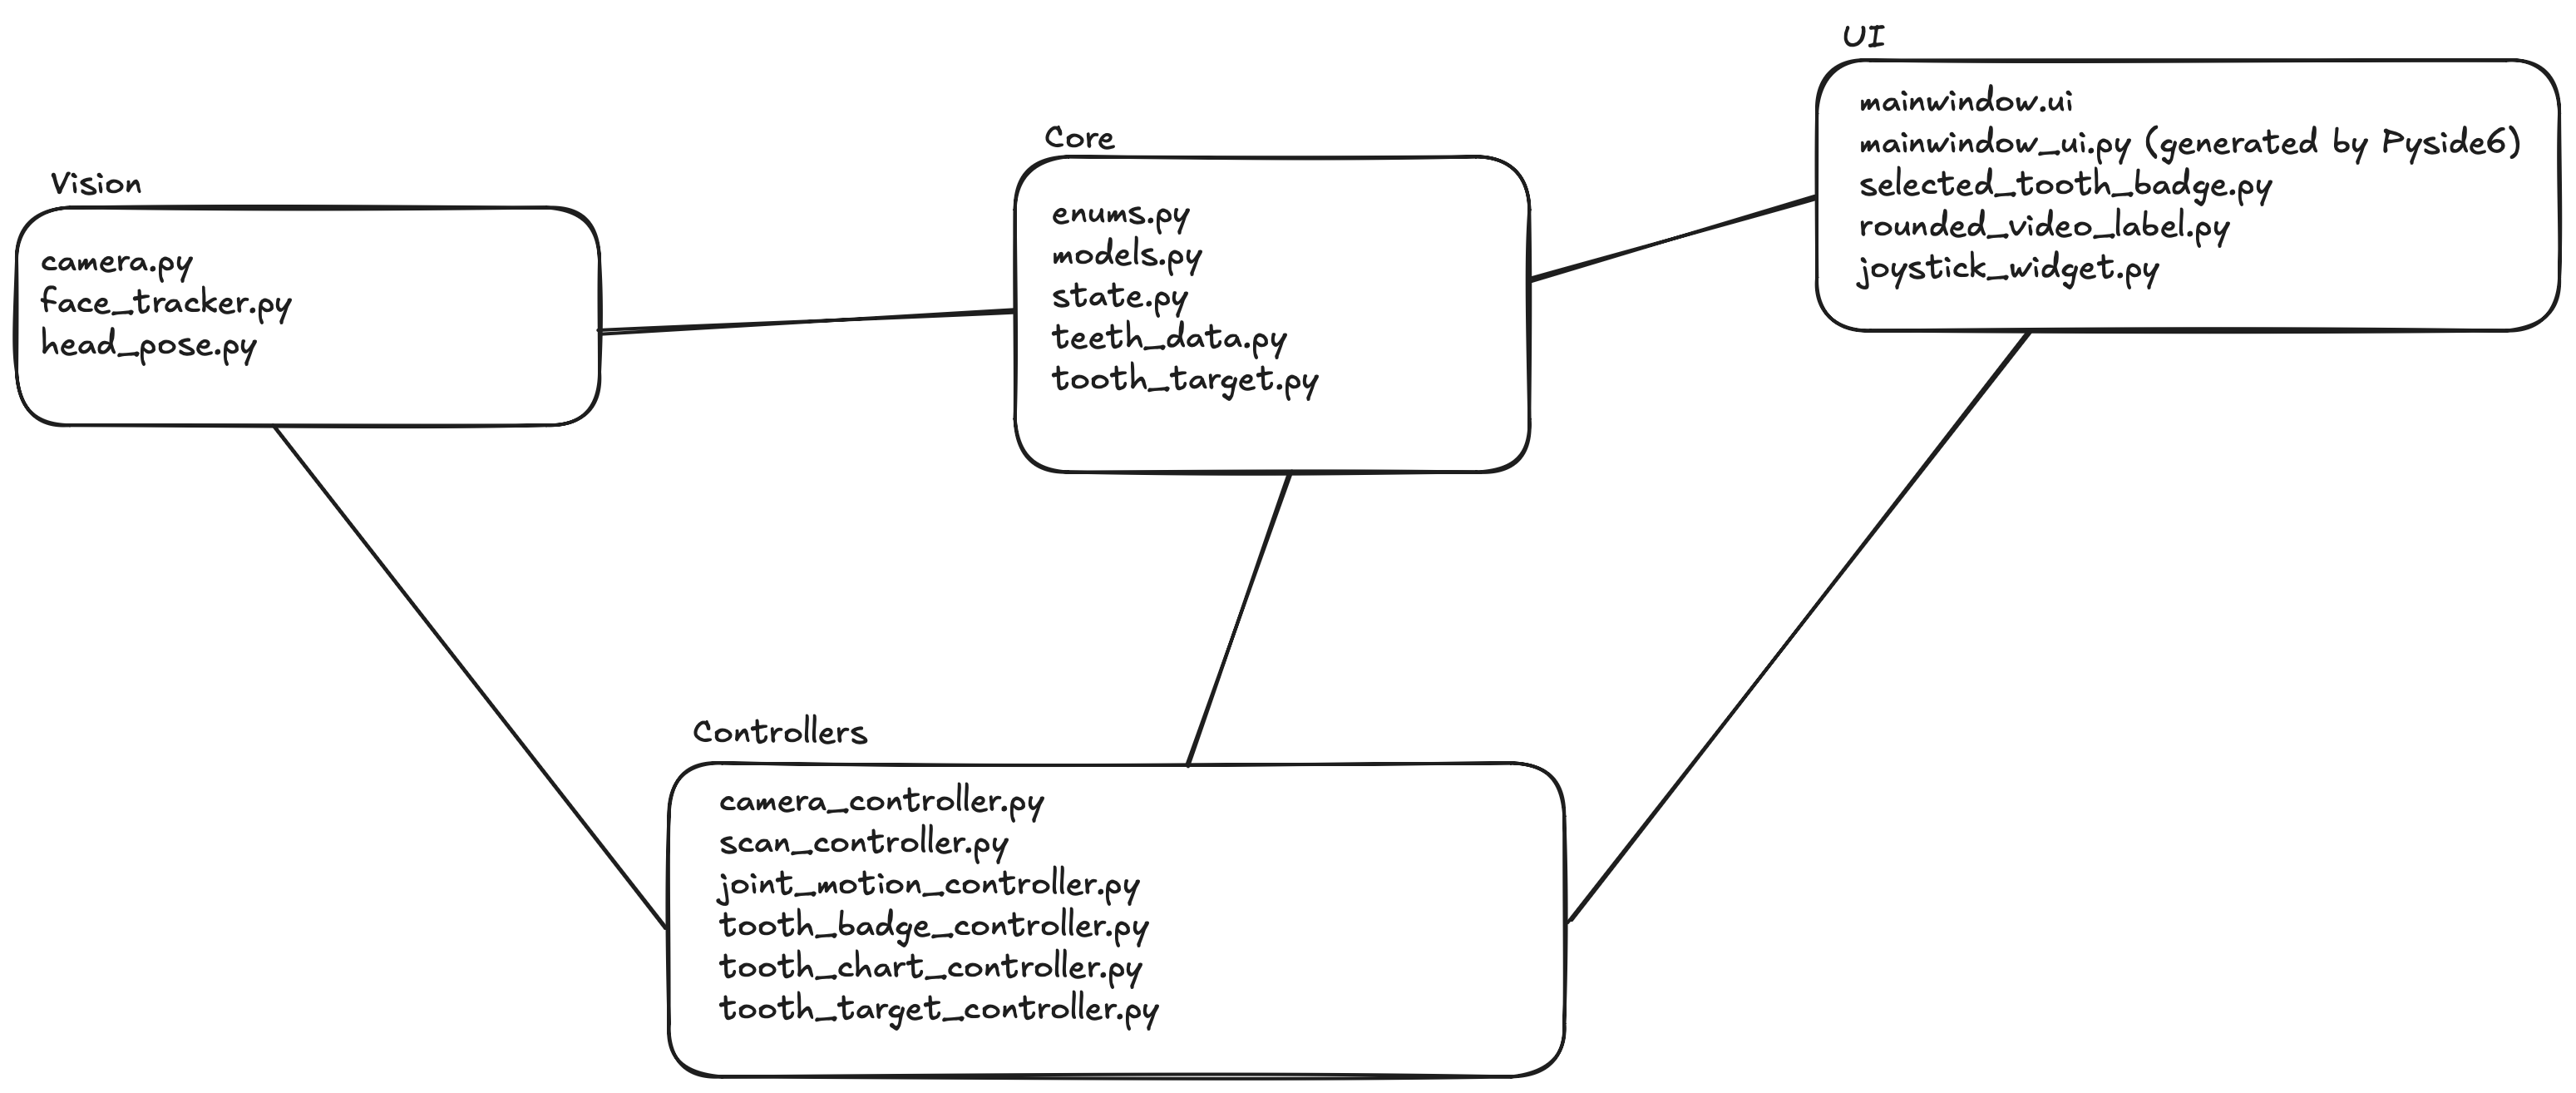
\includegraphics[width=1.1\columnwidth]{ui_assets/overview.png}
    \caption{System Organization Overview drawn in Excalidraw}
    \label{fig:overview}
\end{figure}


\subsection{Data Flow}



\subsection{Dependencies and System Requirements}

The panel logici python ve design qt araciligiyla gelistirildi. Panelde bulunan kamera ve face detection icin OpenCV ve MediaPipe gibi python computer vision kutuphaneleri kullanildi. 
Baslica kullanilan componentleri Tablo~\ref{tab:dependencies}de gorulmektedir.    


\begin{table}[h]
    \centering
    \caption{Dependencies and Development Tools Used in Control Panel}
    \label{tab:dependencies}
    \begin{tabularx}{\columnwidth}{@{}l X@{}}
        \toprule
        \textbf{Component} & \textbf{Purpose} \\
        \midrule
        Python   & Used to implement the application \\
        PySide6 & GUI framework (Qt for Python bindings) \\
        MediaPipe & Face and mouth landmark detection \\
        OpenCV & Camera capture, color conversion, and overlay drawing \\
        Qt Creator & Visual design and layout editing of UI \\
        \bottomrule
    \end{tabularx}
\end{table}

\subsection{Operating Environment and Physical Setup Assumptions}
DentaVision Control Panelin dogru calismasi icin varsayilan fiziksel bir kurulum bulunmaktadir:

\begin{itemize}
    \item Control Paneli touchable bir screen olarak dusunulmustur ve saglik personeli bu paneldeki componentleri dokunmatik olarak kullanir/kontrol eder.
    \item Calisan bir webcam veya USB kamera gereklidir, Mediapipe CPU uzerinde de calisabildiginden GPU gerekli degildir. (bu bilgi gerekli mi?) 
    \item Patient klinikte bulunan sabit bir dental koltukta, kafasi dental head stabilizer ile sabitlenmis bir sekilde oturur. Muayene boyunca kafa poziyosnu fix kalir, asagi yukari veya saga sola hareket etmez.
    \item Koltugun yuksekligi ve kameraya olan mesafesi visionun guvenilirligini etkilemeyecek bir mesafede ayarlanir ve sabit kabul edilir.
    \item Panelde görülen kamera bir konuma sabit monte edilir ve hareket etmez.
    \item Kamera ve Kontrol Panel ayni cihazda bulunabilirken, hasta koltuguna entegre edilen external bir kamera da kullanilabilir.
    \item Odadaki isiklandirma kamera gorus acisi icin optime edilir veya kameranin gordugu alana manuel bir isik eklenmelidir.
\end{itemize}

Bu setuplar ile kamera ve hasta arasi hep sabit bir mesafede oldugu icin HeadPosition.z degeri kameradan olculmez, sabit bir baseline degeri olarak alinir. 
Ayni zamanda, bu sabit olcum sayesinde kameradaki bir pixelin kac cme denk geldigini ifade eden CM\_PER\_PIXEL kalibrasyon sabiti tek bir ölcümle belirlenebilir ve tooth targetin hastanin agiz boyutuna daha uyumlu calismasi hedeflenmektedir.
Koltuk veya kamera yeri degisirse yeniden kalibrasyon gerekmektedir. 

\section{User Interface Design}
Control panel UI Designinda MEdical ortama ve personal user experiencei icin user flow Figure~\ref{fig:userflow} dusunulup olabildigince optimal bir sekilde gerceklestirilmeye calisilmistir. 


\begin{figure}[t]
    \centering
    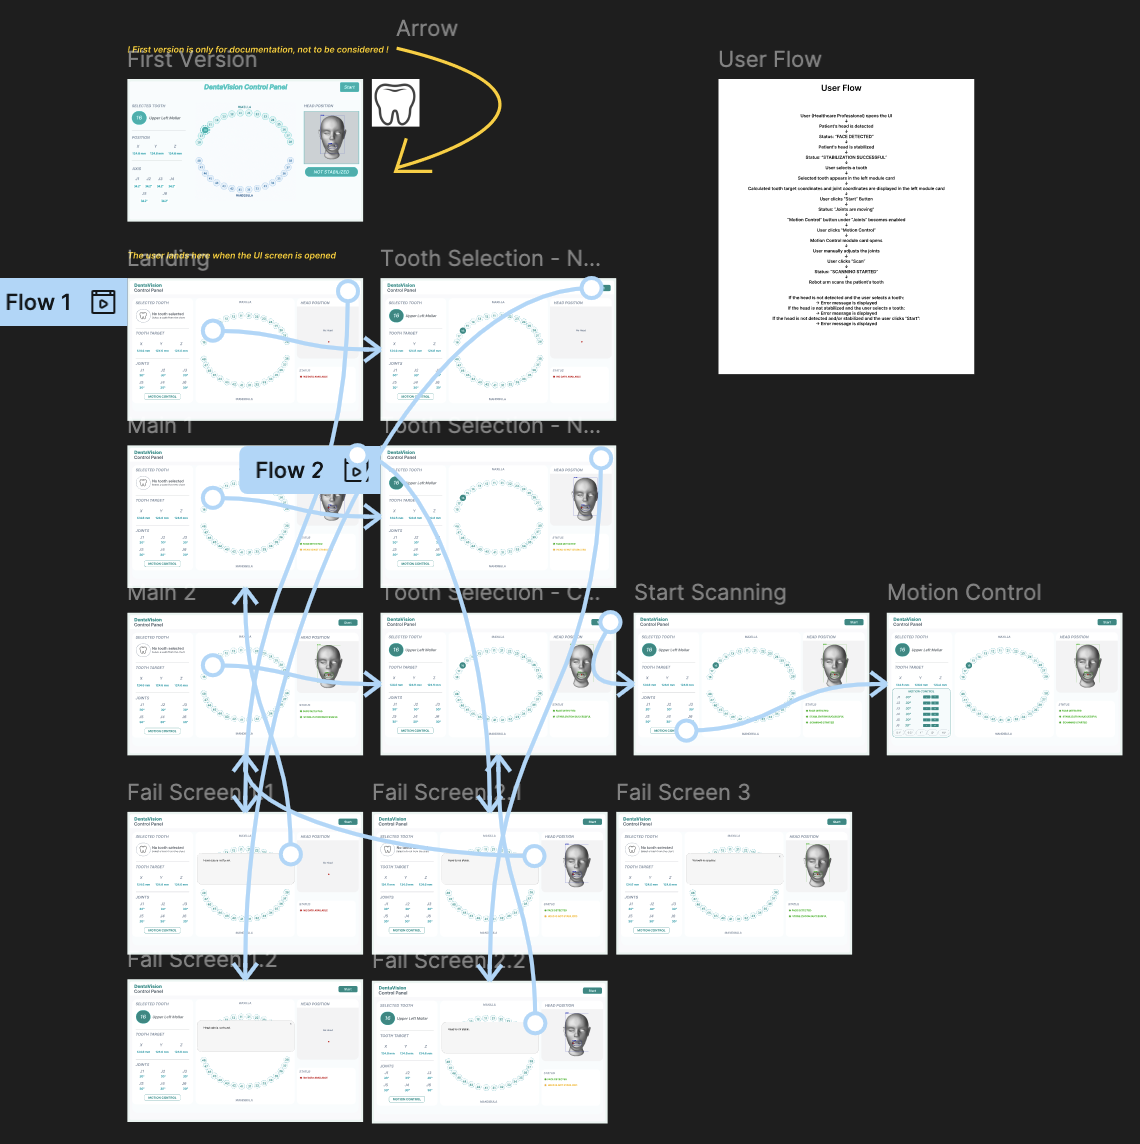
\includegraphics[width=\columnwidth,height=0.45\textheight,keepaspectratio]{ui_assets/figma_.png}
    \caption{Figma Control Panel UI Design Layout}
    \label{fig:userflow}
\end{figure}

Baslangicta daha basit bir user flow baz alinarak Figma da design ilk versiyonu Figure ~\ref{fig:figma} olusturulmustur ve sonrasinda iterasyonla bu dizayn iyilestirilip implementasyon asamasinda optimize edilmeye devam edilmistir.

\begin{figure}[t]
    \centering
    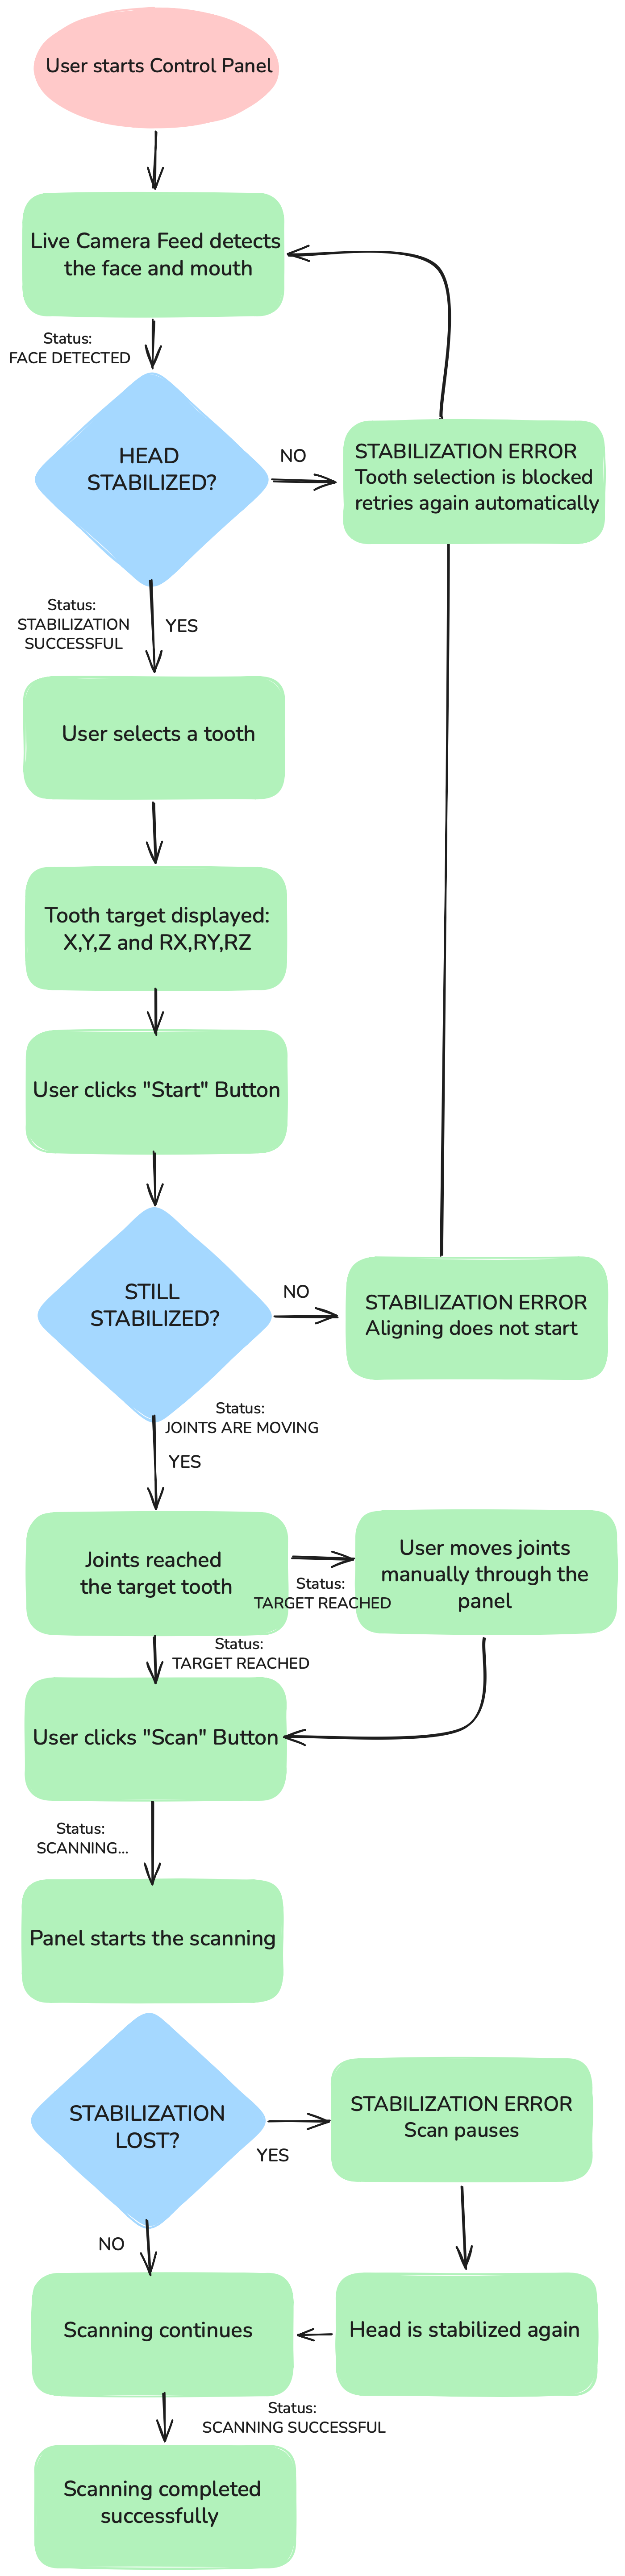
\includegraphics[width=\columnwidth,height=0.45\textheight,keepaspectratio]{ui_assets/user_flow.png}
    \caption{User Flow Diagramme (Excalidraw)}
    \label{fig:figma}
\end{figure}

Bu baglamda su designda su noktalara dikkat edilmistir: 

\begin{itemize}
    \item AA
\end{itemize}

Design Qt Creator ui dosyasi olusturup Layoutlar, Frameler, QLabellar etc. ile dizayn edilmistir. Figure~\ref{fig:qt}
Joystick widget gibi bazi ui componentleri complex olmalari nedeniyle py dosyasi ile olusturulmustur.


\begin{figure}[t]
    \centering
    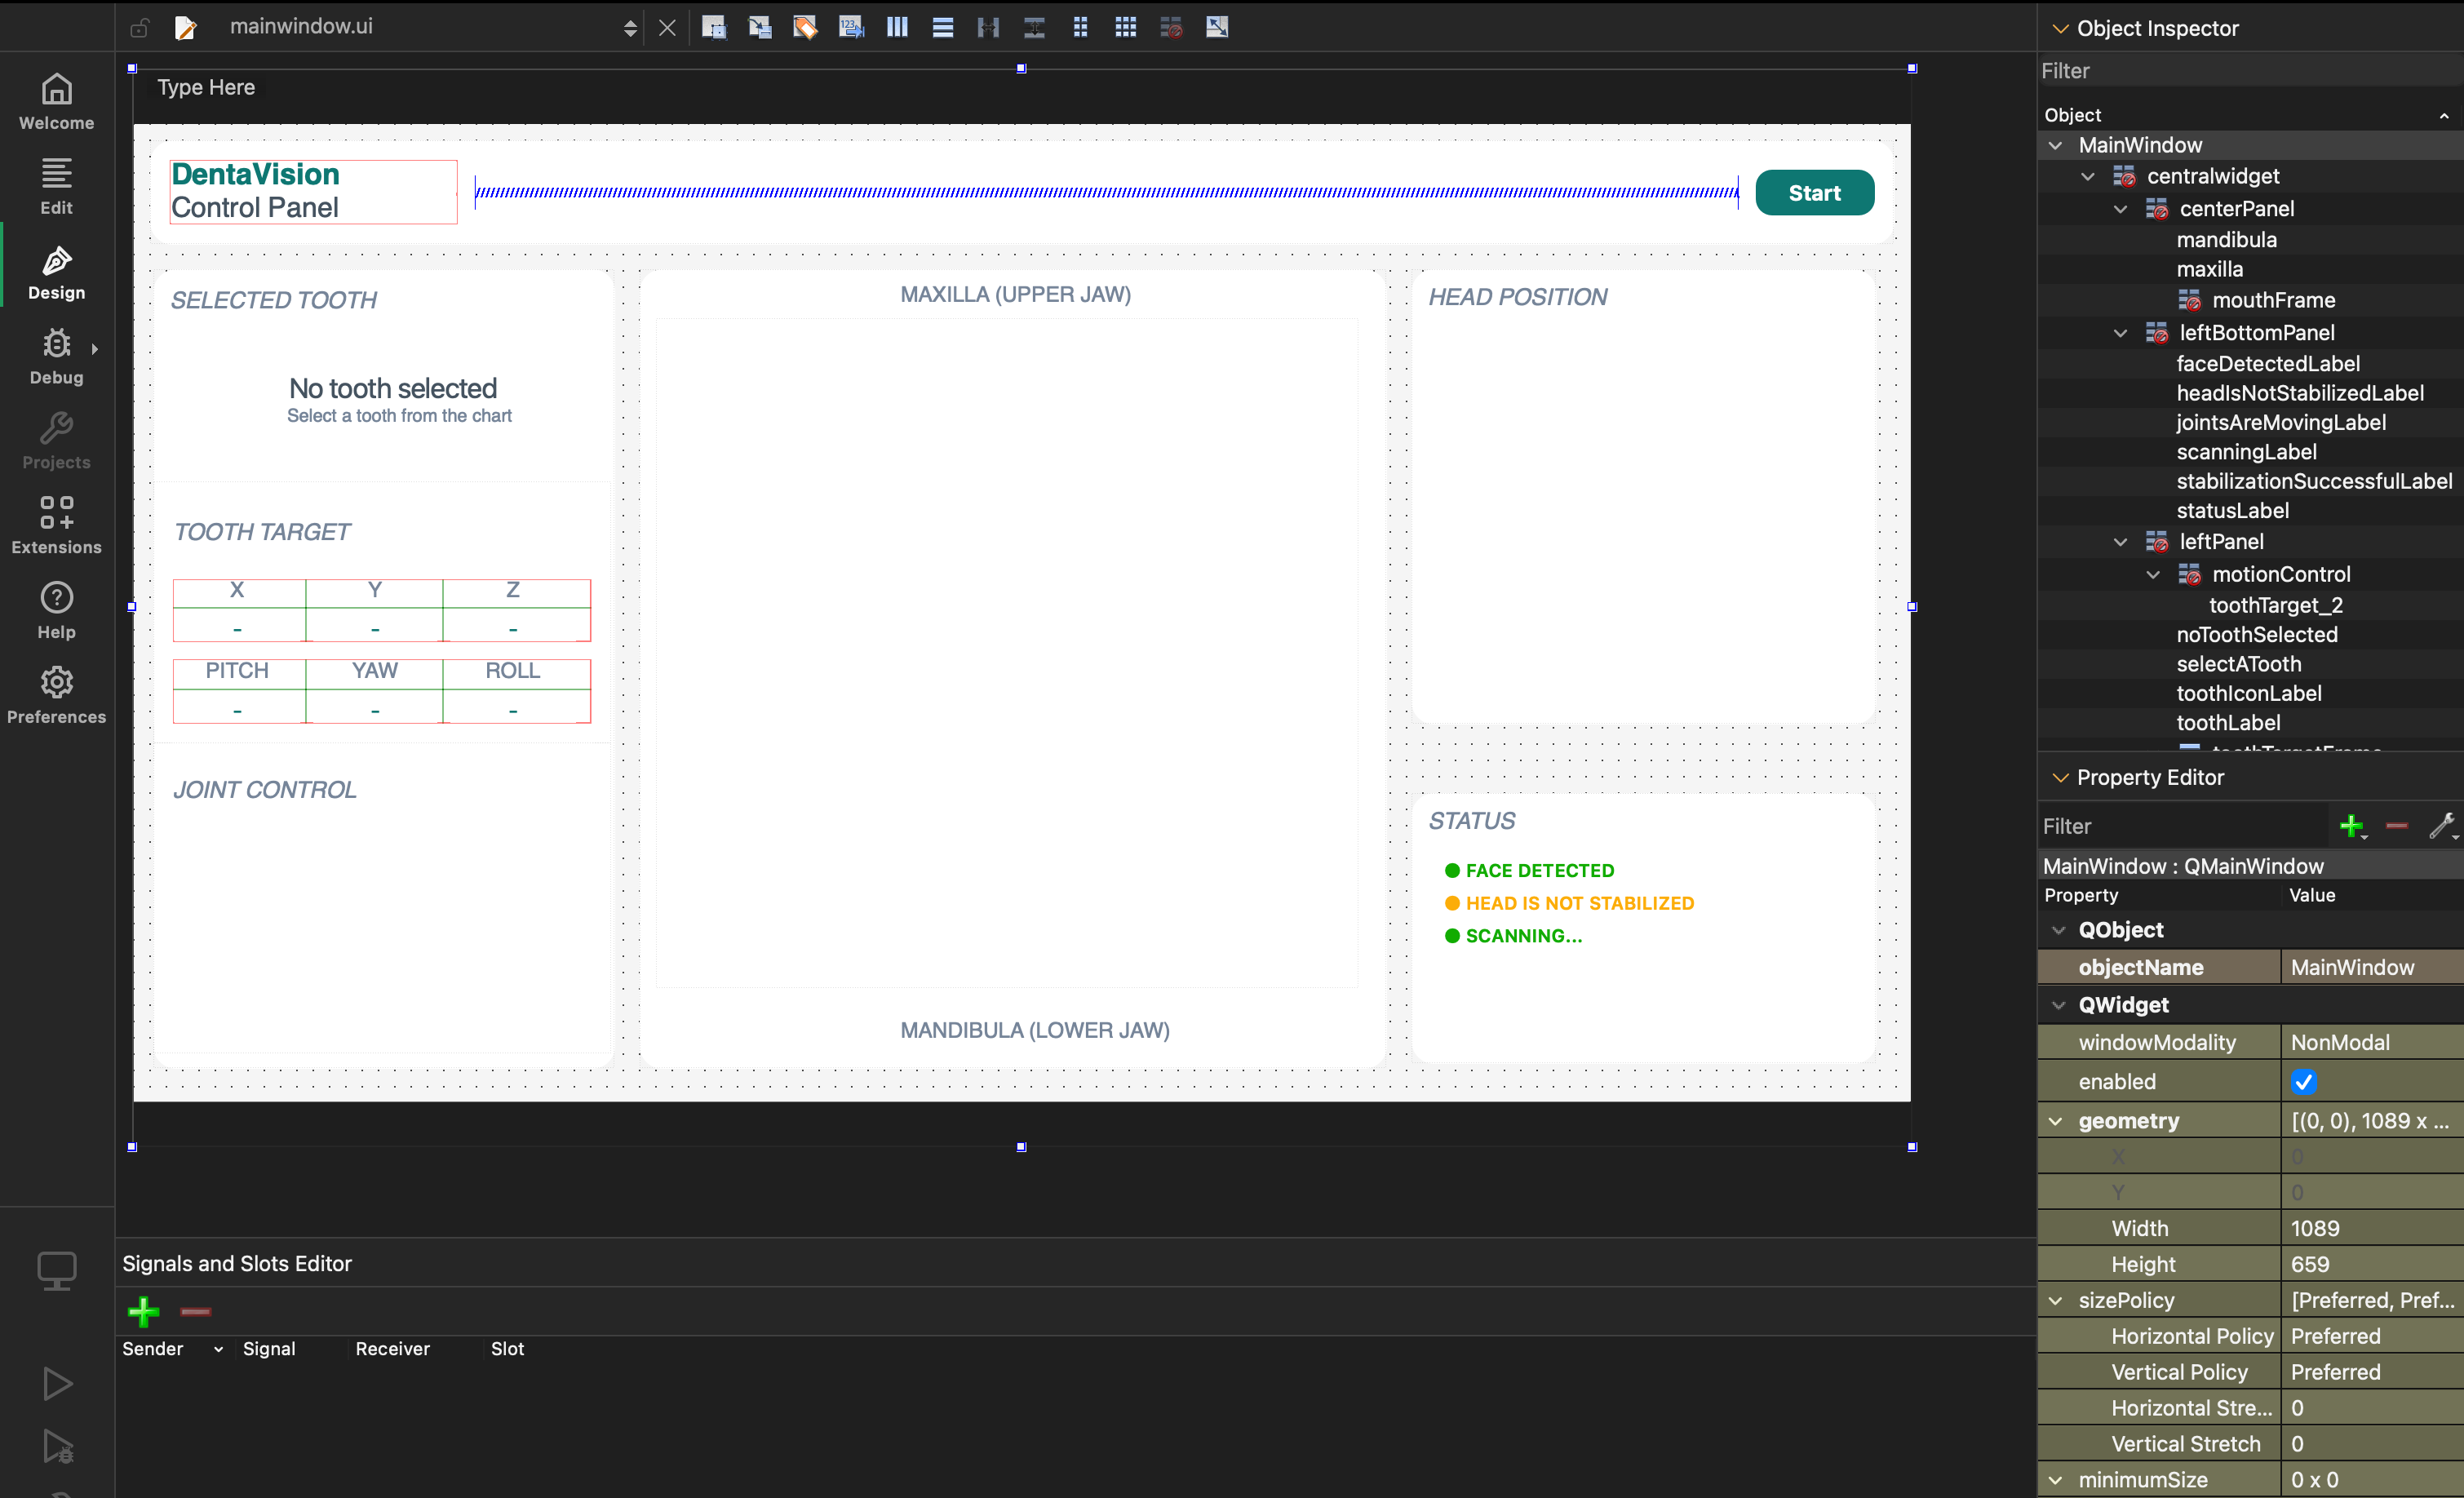
\includegraphics[width=\columnwidth,height=0.45\textheight,keepaspectratio]{ui_assets/qt.png}
    \caption{Qt Creator UI File}
    \label{fig:qt}
\end{figure}

\begin{figure}[t]
    \centering
    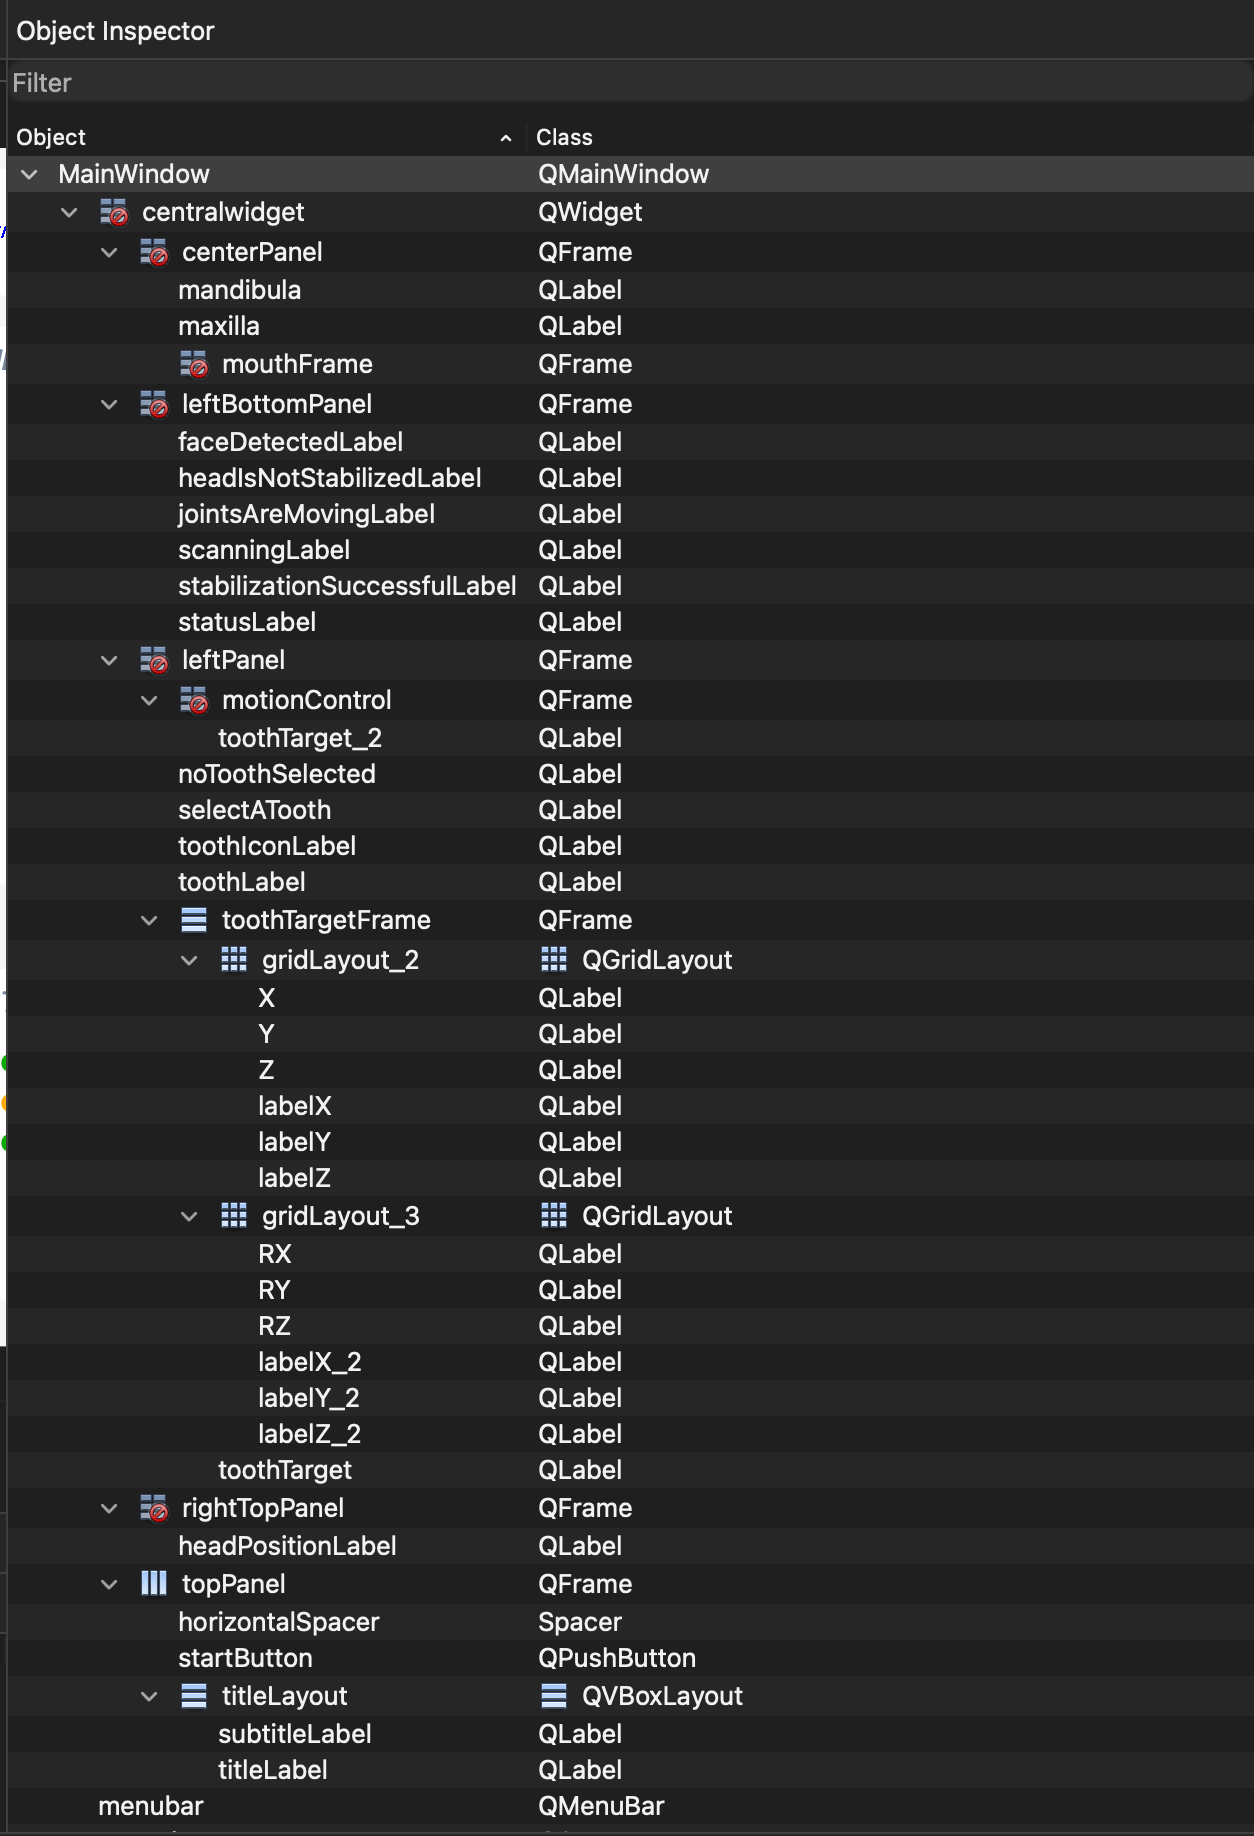
\includegraphics[width=\columnwidth,height=0.35\textheight,keepaspectratio]{ui_assets/object_inspector.png}
    \caption{Qt Creator Object Inspector}
    \label{fig:object_inspector}
\end{figure}

\subsection{Main Window Layout}
Main Window, islem akisini soldan saga ve ustten alta okunacak sekilde 3 panele böler: Solda sirasiyla ustten alta dis secim gostergesi, secilen dis icin tooth targeting sonuclarinin degerleri ve personelin manuel olarak joint hareketlerini kontrol edebilecegi bir motion control modulu bulunmaktadir.
Ortada ise hedeflenen disin secilmesine olanak saglayan tooth chart paneli bulunmaktadir ve son olarak sagda, canli kamera goruntusu ve sistem stateini gosteren status paneli olmak uzere iki panel bulunmaktadir.
En ustte layoutta ise Control Panelin logosu ve 3 asamali Start/Scan/Pause butonu bulunur. 

Main Window ilk once Figma'da ilk versiyonu Figure~\ref{fig:mainwindow_first} olusturulmustur. Bu layout supervisor feedbackleri ve gelisen proje degisiklikleriyle use case ve gercek hayat usabilitysine yonelik revize edilmistir. Figure~\ref{fig:mainwindow_current}

\begin{figure}[h]
    \centering
    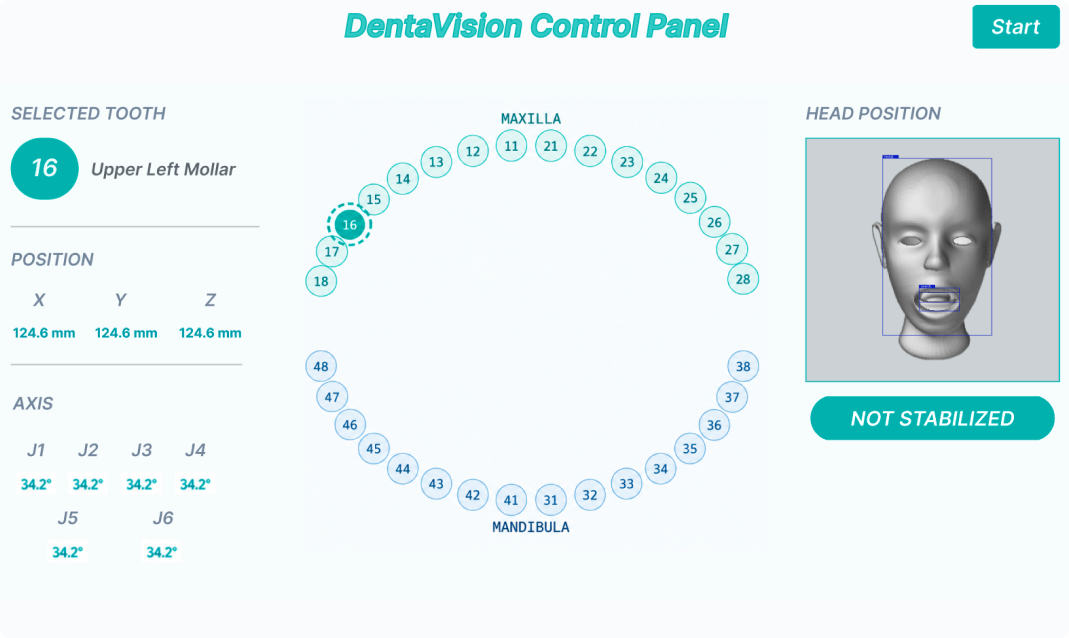
\includegraphics[width=\columnwidth,height=0.40\textheight,keepaspectratio]{ui_assets/first_version.png}
    \caption{First Version of MainWindow}
    \label{fig:mainwindow_first}
\end{figure}

Güncel:

\begin{figure}[h]
    \centering
    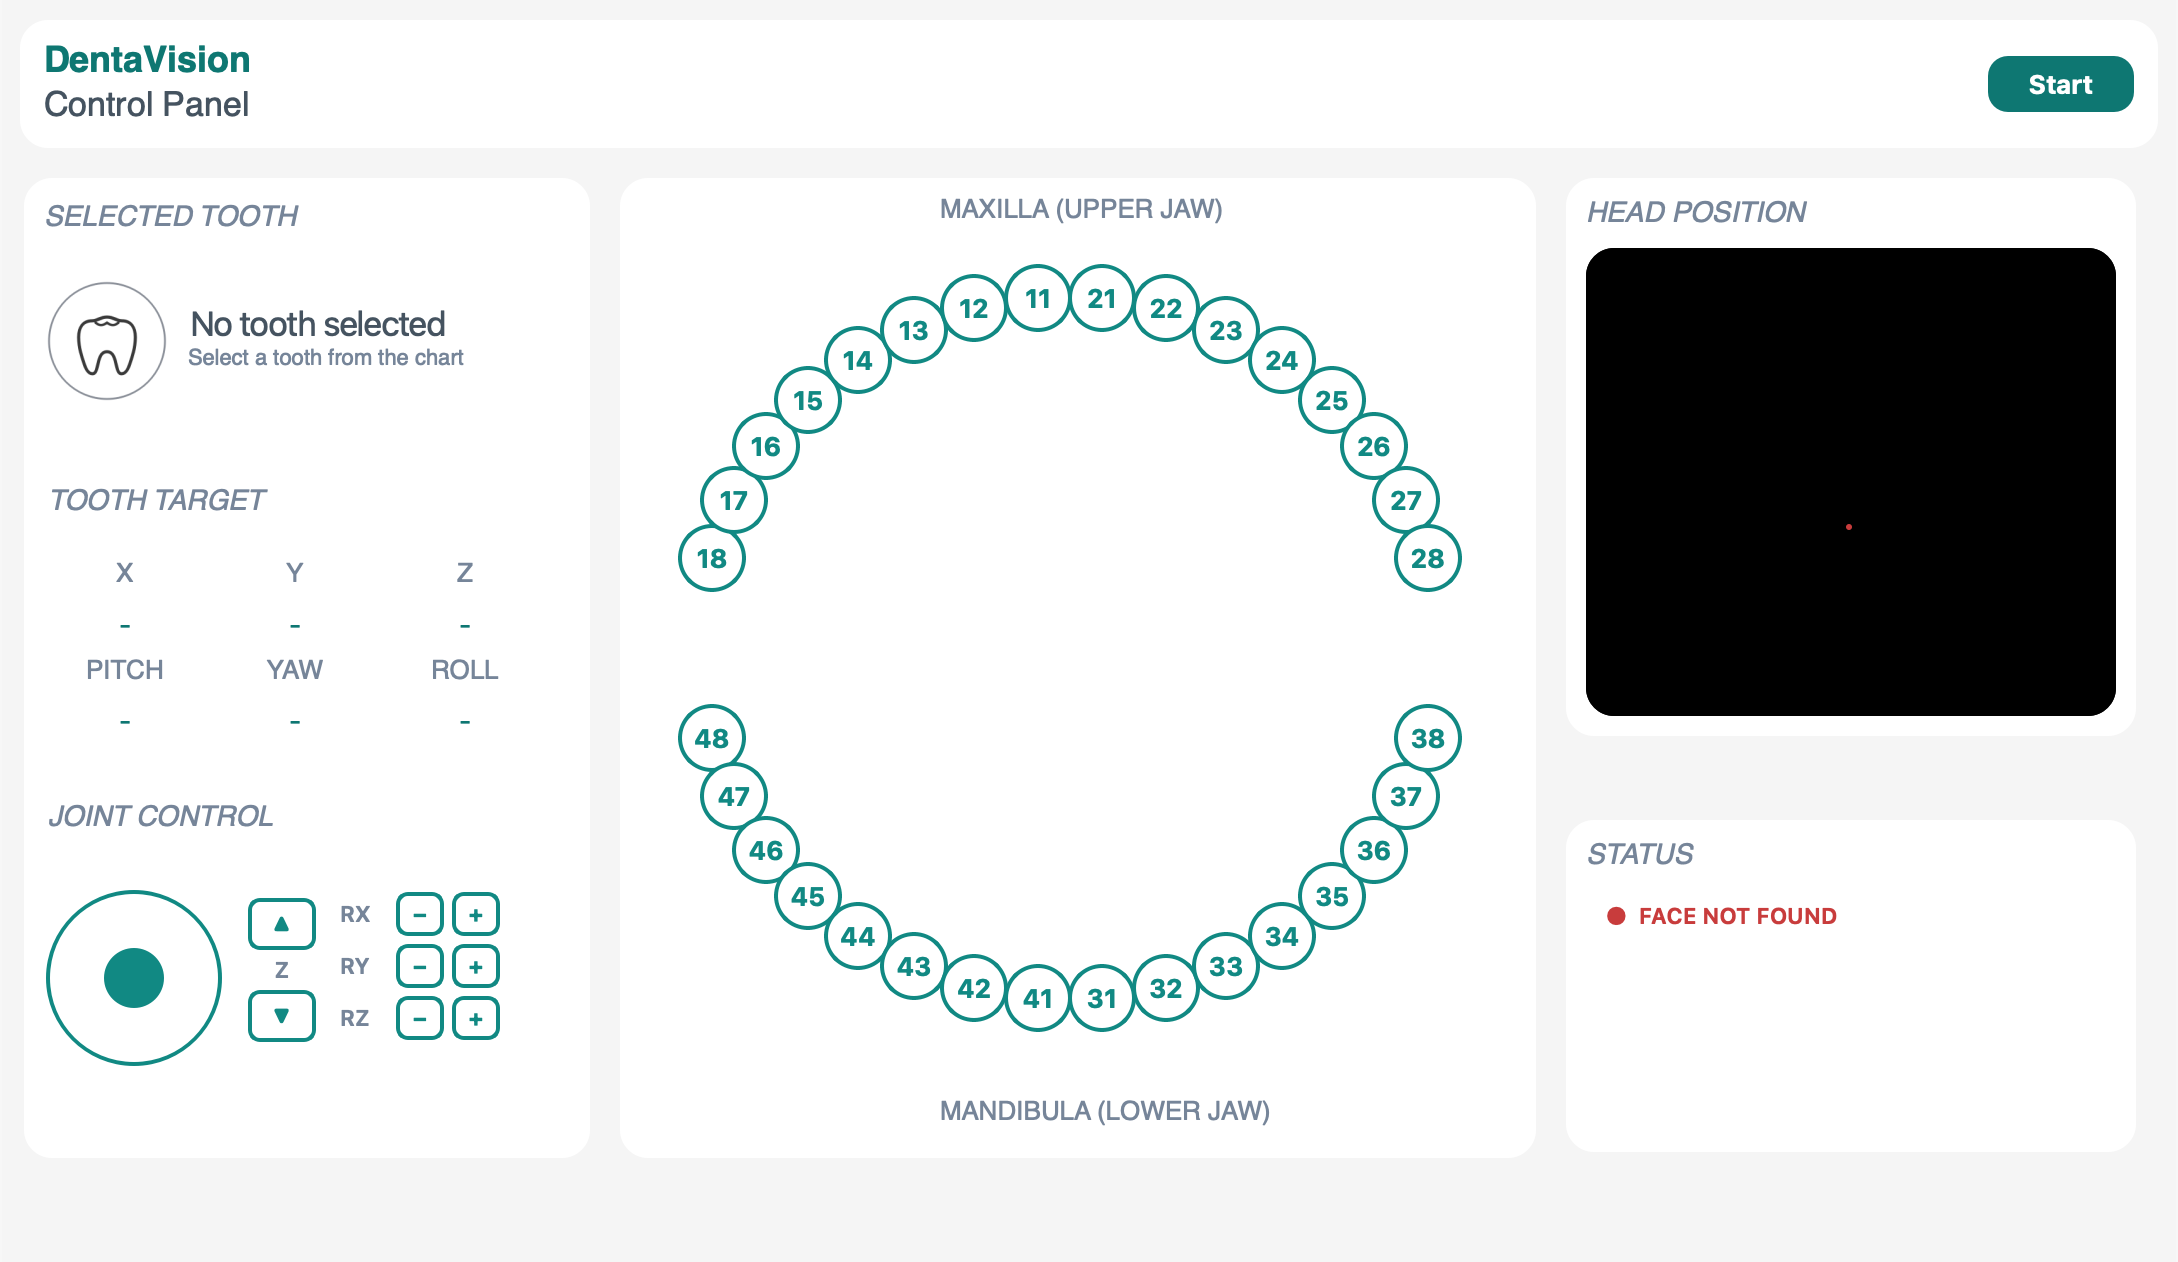
\includegraphics[width=\columnwidth,height=0.40\textheight,keepaspectratio]{ui_assets/current_ui_oP.png}
    \caption{Last Version of MainWindow}
    \label{fig:mainwindow_current}
\end{figure}

\subsection{Tooth Target Panel}

Bu panel 'selected tooth' altinda default (no tooth selected) dis figuru seklinde bir logo bulundurur Figure~\ref{fig:no_tooth_selected_badge}. 
Dental archtan bir dis secildiginde bu figur yerine secilen disin FDI numarasi gelir ve ismi yaninda yazdirilir. Figure~\ref{fig:tooth_selected_badge} 

\begin{figure}[h]
    \centering
    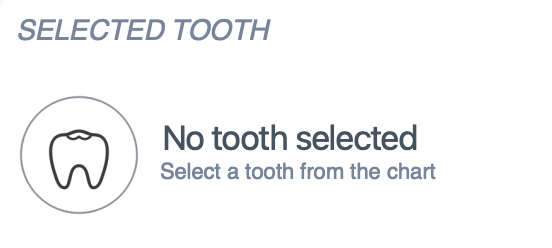
\includegraphics[width=\columnwidth,height=0.40\textheight,keepaspectratio]{ui_assets/components/no_tooth_selected.png}
    \caption{No Tooth Selected Badge}
    \label{fig:no_tooth_selected_badge}
\end{figure}

\begin{figure}[h]
    \centering
    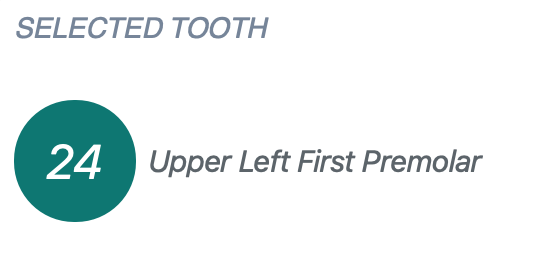
\includegraphics[width=\columnwidth,height=0.40\textheight,keepaspectratio]{ui_assets/components/tooth_selected.png}
    \caption{Tooth Selected View}
    \label{fig:tooth_selected_badge}
\end{figure}

Selected Tooth bolumunun altinda Tooth Target alani bulunur. Bu alan secilen dise gore hesaplanan hedef koordinatları, konum icin X,Y,Z ve rotation icin pitch, roll, yaw degerlerini panel kullanicisina gosterir.
Hicbir dis secilmemisken tum etiketlerin '-' olarak gosterilmesi tercih edilmistir. Figure\ref{fig:tooth_target_} bu, "henüz hesaplanmış geçerli bir değer yok" durumunu "0.0 mm" gibi hesaplanmış bir değerle karıştırmayı önleyen bilinçli bir tercihtir, çünkü 0.0 mm operatör tarafından gerçek bir ölçüm sonucu sanılabilir.
Ekrandan bir dis secildiginde etiketler, birimleriyle birlikte anlik olarak guncellenir. \ref{}    
 
\begin{figure}[h]
    \centering
    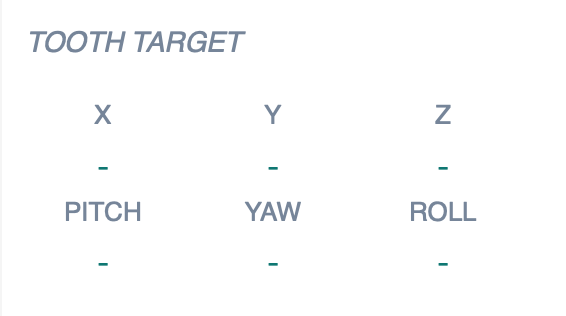
\includegraphics[width=\columnwidth,height=0.40\textheight,keepaspectratio]{ui_assets/components/tooth_target_.png}
    \caption{Tooth Target Landing/Default View}
    \label{fig:tooth_target_}
\end{figure}

\begin{figure}[h]
    \centering
    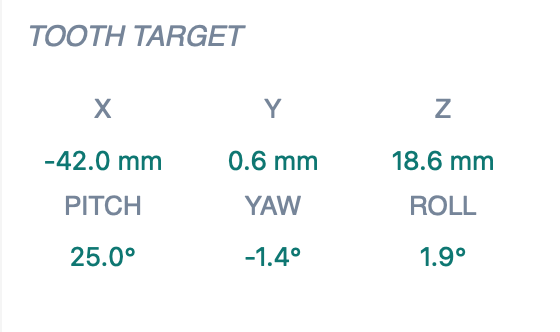
\includegraphics[width=\columnwidth,height=0.40\textheight,keepaspectratio]{ui_assets/components/tooth_target.png}
    \caption{Tooth Target View}
    \label{fig:tooth_target}
\end{figure}


\subsection{Manuel Joint Control Panel}

sistem su ..... asamalardayken kullanima aciktir. Manuel motion kontrol ayari yapilabilir.

\begin{figure}[h]
    \centering
    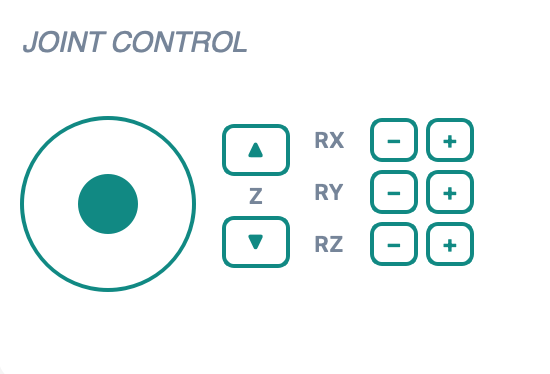
\includegraphics[width=\columnwidth,height=0.40\textheight,keepaspectratio]{ui_assets/components/joint_control.png}
    \caption{Joint Control Panel}
    \label{fig:joint_control}
\end{figure}

BURAYA TERMINAL CIKTISI DA EKLE 

Joint adjustments su caselerde yapilabilmektedir:

\begin{itemize}
    \item A
\end{itemize}

\subsection{Tooth Chart Panel}

Dis secim paneli, disleri duz bir liste veya tablo olarak degil, conceptul basitlestirilmis dental bir arkin (ust ve alt cene yayinin) geometrisine benzer eliptik bir duzen uzerinde konumlandirir. Figure~\ref{fig:dental_arch} 
Panelde dental arki anlamayi kolaylastiran maxilla (upper jaw) ve mandibula (lower jaw) labellari bulunmaktadir.
Bu tasarim personelin gorsel olarak disi daha hizli ve sezgisel bulmasina yardimci olmayi ongormektedir. Bu sayisal bir listeye gore cognitive load belirgin bir sekilde azaltir. 

\begin{figure}[h]
    \centering
    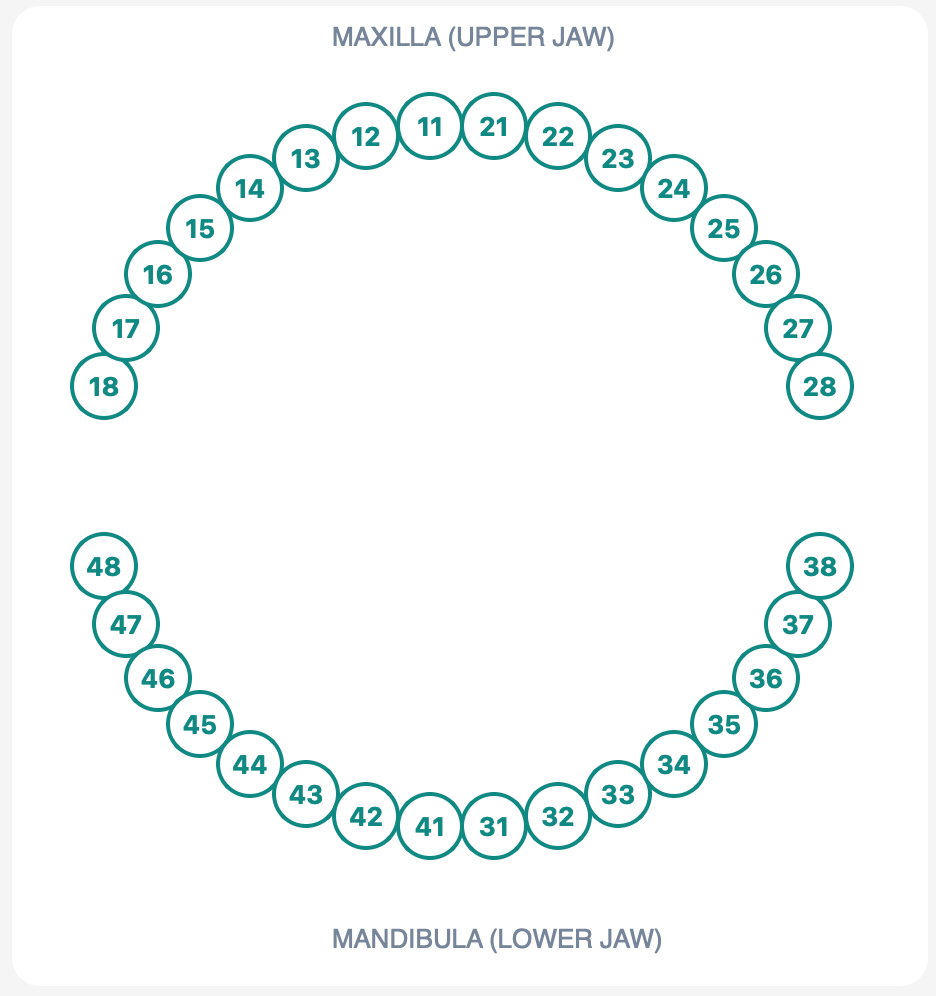
\includegraphics[width=\columnwidth,height=0.40\textheight,keepaspectratio]{ui_assets/components/dental_arch.png}
    \caption{Dental Arch Landing View}
    \label{fig:dental_arch}
\end{figure}

Bir dise tiklandiginda, (on\_tooth\_selected) hastanin kafa pozisyonu yeterince stabilse secilen disin ismi ve FDI numarasi bir badge Figure~\ref{fig:dental_arch_chosen} olarak gorunur.
Kafa pozisyonu yeterince stabil degilse sistem secimi bastan engeller, bu sayede hastanin kafasi hareket halindeyken guvenilir olmayan bir Tooth Target uzerinde calisilmasinin onune gecilmesi ongorulur.
Bu casein error mesaji terminale yazdirilirken, gercek hayattaki karsiliginda panelde secime izin verilmez ve Status olarak "head not stabilized" notificationu sayesinde personel bunun bilincine varir.  


\begin{figure}[h]
    \centering
    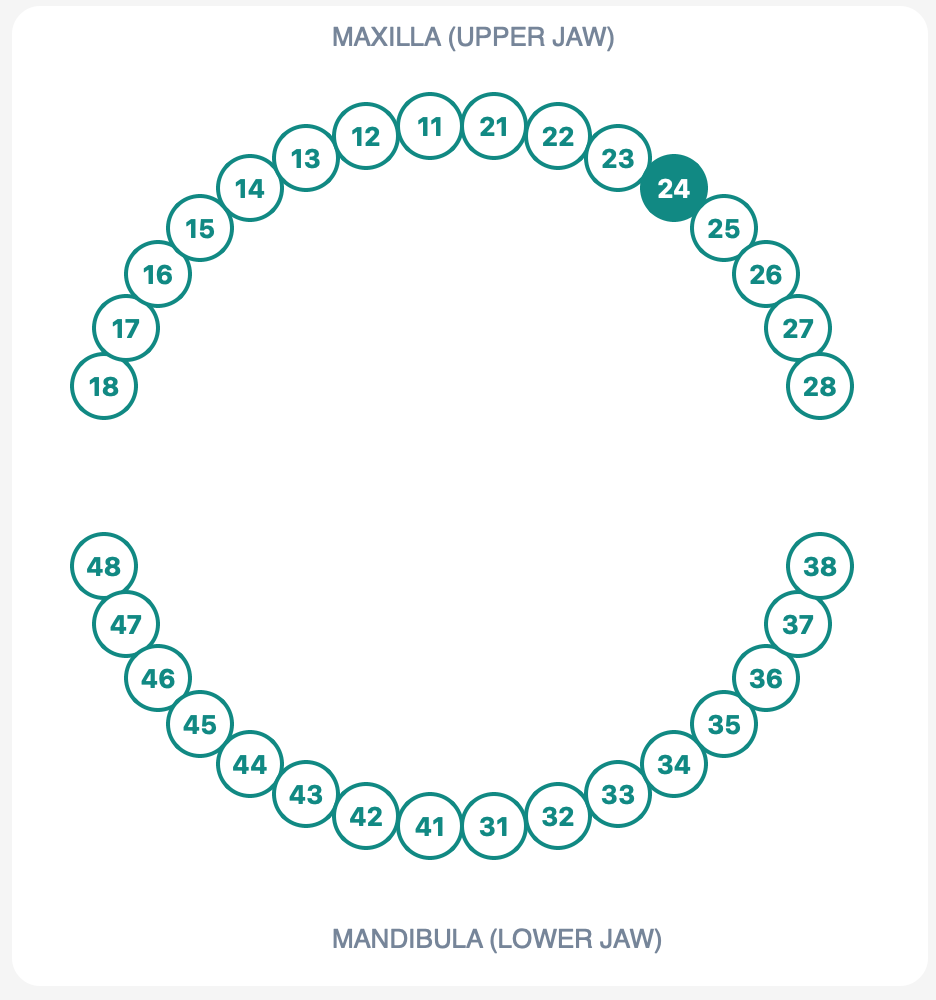
\includegraphics[width=\columnwidth,height=0.40\textheight,keepaspectratio]{ui_assets/components/dental_arch_chosen.png}
    \caption{Dental Arch Tooth Chosen View}
    \label{fig:dental_arch_chosen}
\end{figure}

\subsection{Camera Panel and Status Indicators}

The Camera Panel consists of a live video feed with bounding boxes highlighting the detected face and mouth, with rounded corners framing the detected regions. Figure~\ref{fig:camera} illustrates the interface. In addition, a red point is displayed on the screen to indicate the target position at which the patient's mouth should be centered. This visual reference is intended to assist in monitoring the stability of the patient's head position. A default positional tolerance of 15 pixels is defined around the target point;
 therefore, the patient's mouth is considered to remain within the acceptable stabilization range when its detected position stays within this tolerance.
Tespit durumuna gore FACE NOT FOUND \ref{}, FACE DETECTED \ref{}, STABILIZATION SUCCESSFUL \ref{}, STABILIZATION ERROR \ref{} etiketleri, renk kodlamasiyla desteklenir ve status bolumunde gosterilir.

\begin{figure}[h]
    \centering
    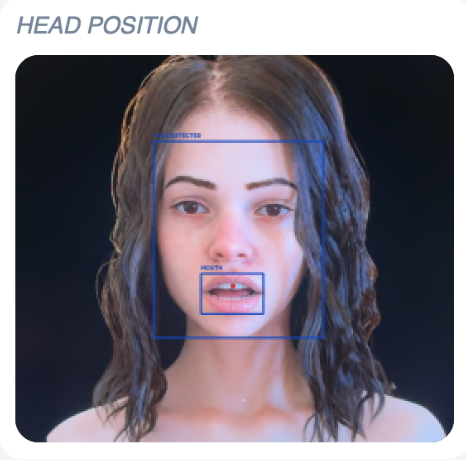
\includegraphics[width=\columnwidth,height=0.40\textheight,keepaspectratio]{ui_assets/components/camera.png}
    \caption{Camera View with a Human Face Model generated by AI. (Status: Head is not stabilized)}
    \label{fig:camera}
\end{figure}


Start butonuna tiklanilarak jointlere hareket komutu verildikten sonra sirasiyla JOINTS ARE MOVING \ref{} ve TARGET REACHED \ref{} etiketleri statuste belirir.
Sonrasinda kullanici gerekli tatbikleri yaptiktan sonra Scan butonuna basar ve sorunsuz ilerlerse statuste sirasiyla SCANNING... \ref{} ve SCANNING SUCCESSFUL \ref{} belirir. 


Status bolumu Camera panelinin hemen altinda bulunur ve personelin sistemdeki akisi ve hastanin guvenligini kontrol etmesine katkida bulunan bir gostergec olarak dusunulmustur.
Status barinin akis hikayesi su sekildedir:

\begin{enumerate}
    \item default olarak kirmizi renkte FACE NOT FOUND etiketi ile baslar. 
    \item Kamerada bir yuz detect edildiginde yesil FACE DETECTED etiketi status barina eklenir.
    \item Eger hastanin kafasi 
\end{enumerate}




\subsection{Buttons}

\begin{figure}[h]
    \centering
    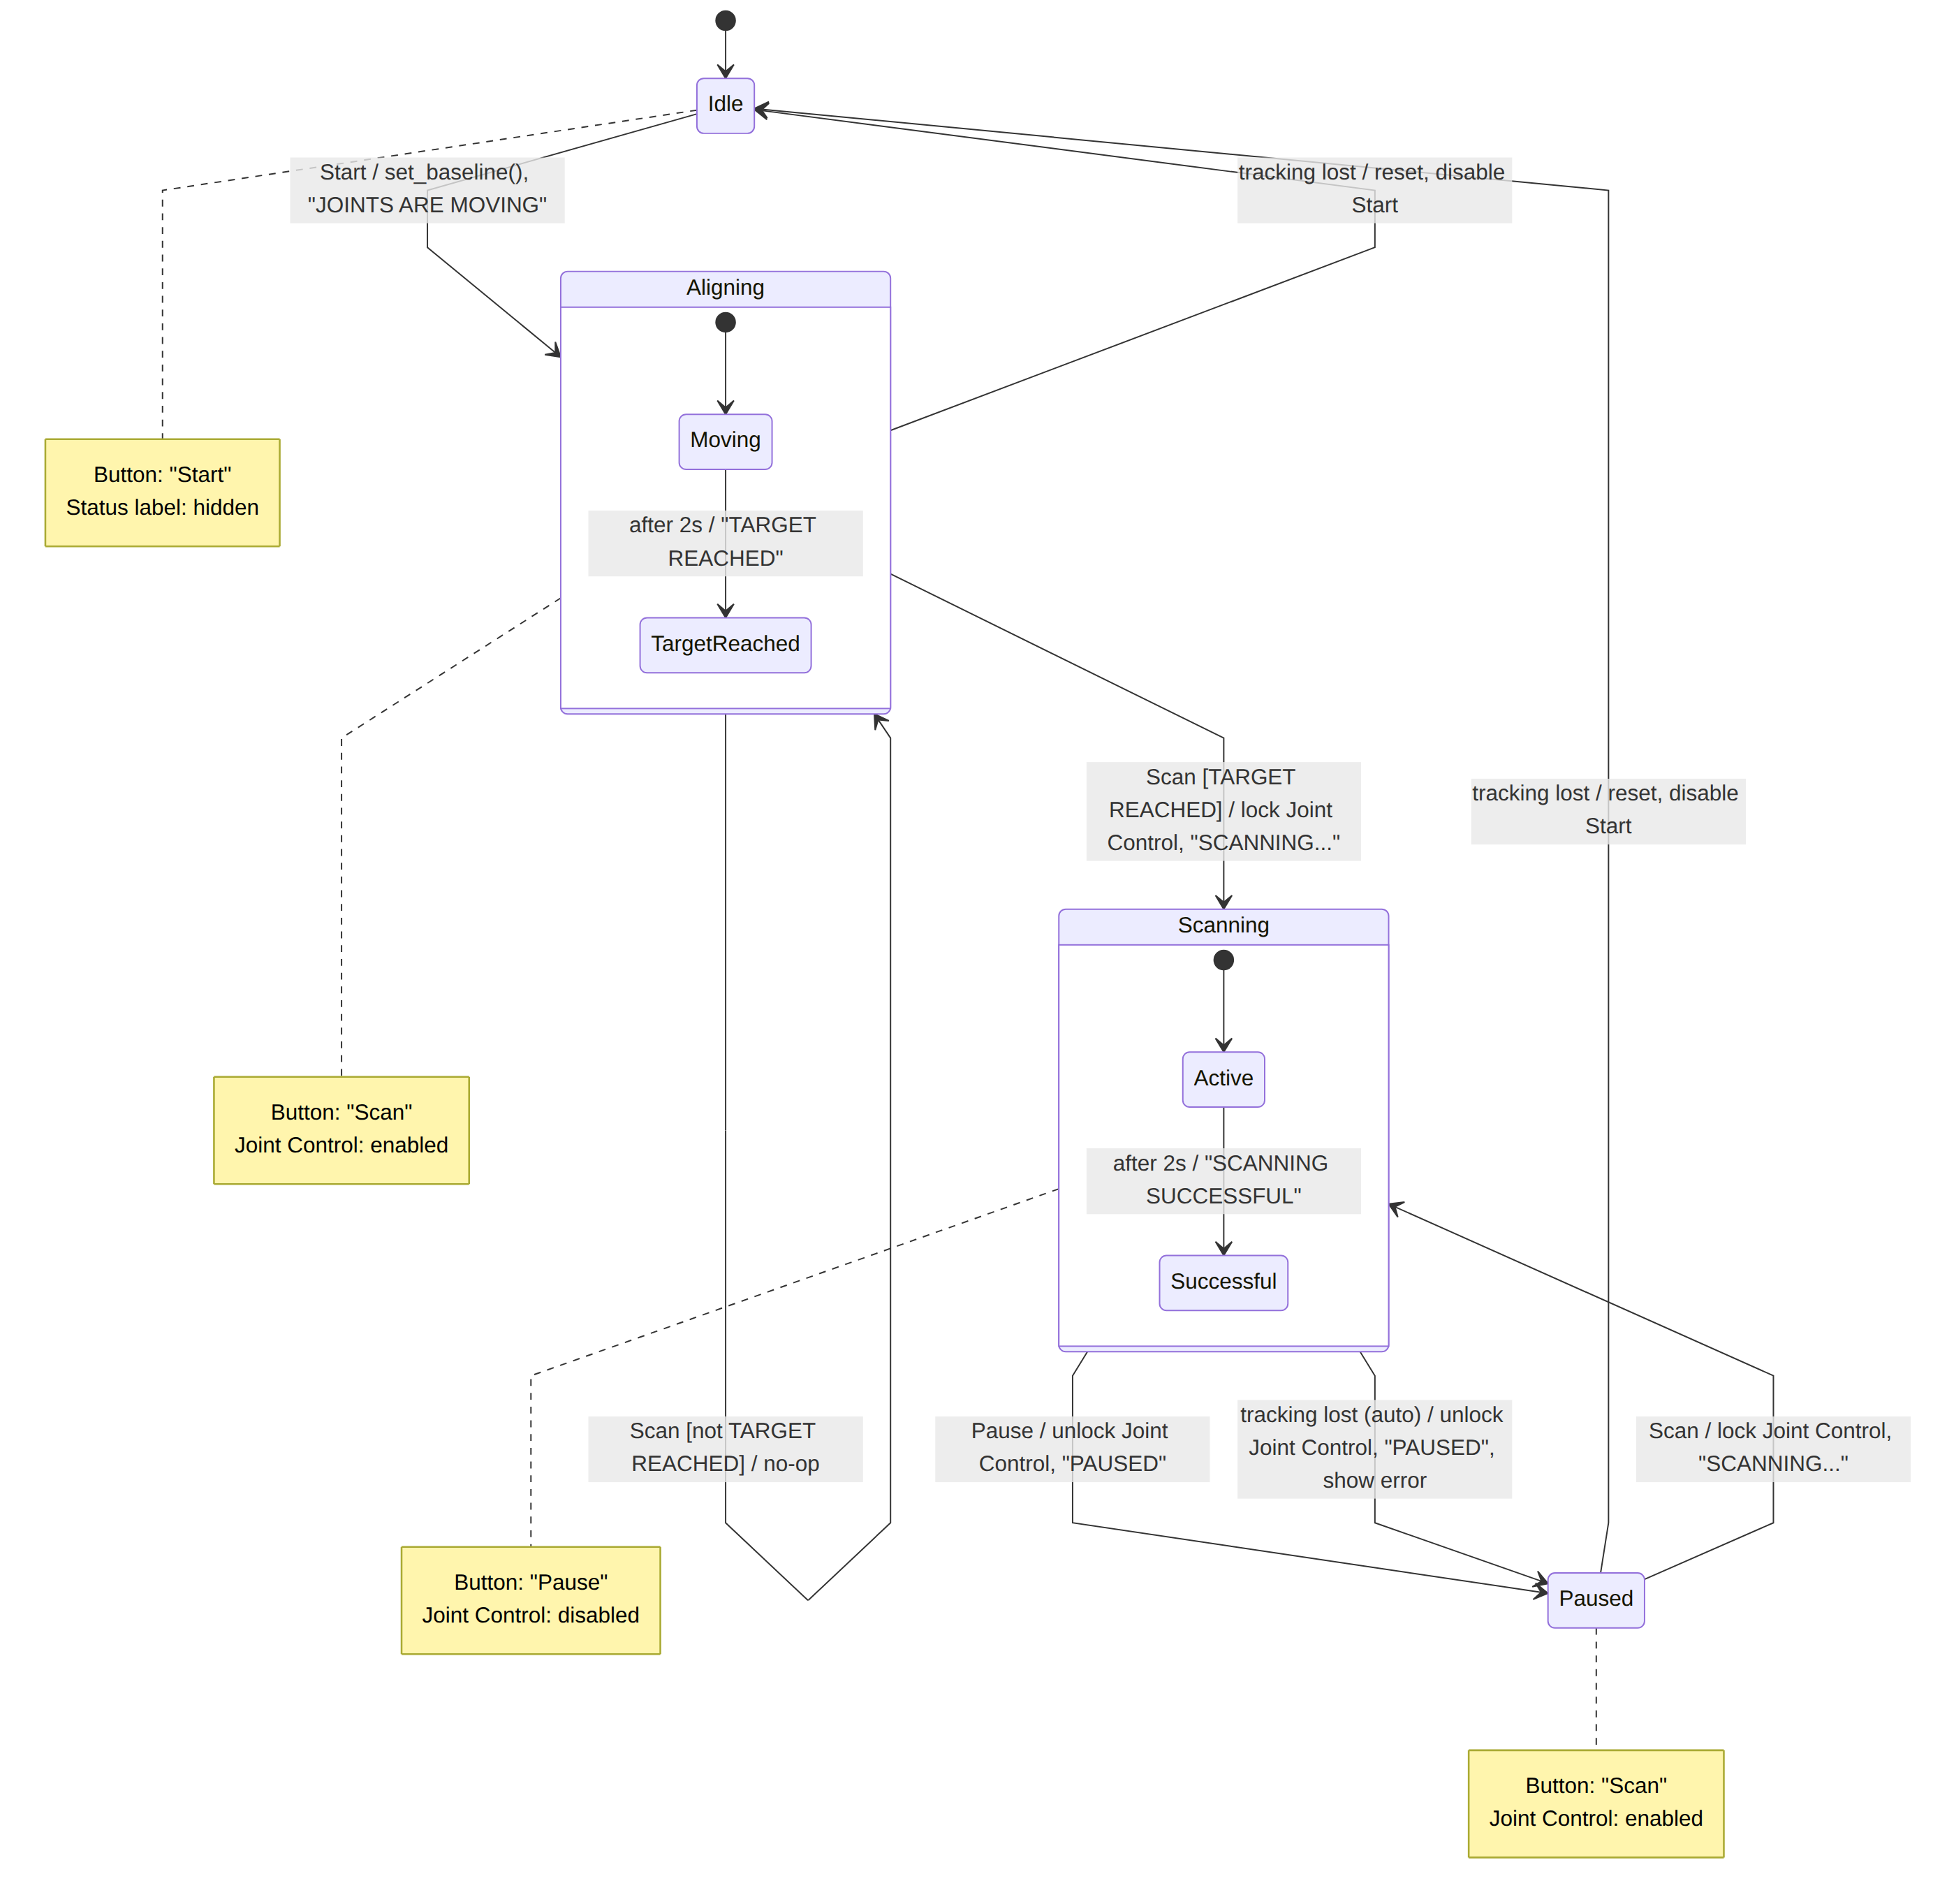
\includegraphics[width=\columnwidth,height=0.45\textheight,keepaspectratio]{ui_assets/state_buttons.png}
    \caption{State Diagram of Button Transformation created by Claude AI}
    \label{fig:buttons}
\end{figure}

\begin{figure}[h]
    \centering
    
\includegraphics[width=0.45\columnwidth,height=0.45\textheight,keepaspectratio]{ui_assets/components/button_start.png}
    \caption{Start Button View}
    \label{fig:button_start}
\end{figure}

\begin{figure}[h]
    \centering
    
\includegraphics[width=0.45\columnwidth,height=0.45\textheight,keepaspectratio]{ui_assets/components/button_start_faded.png}
    \caption{Start Button Faded View}
    \label{fig:button_start_faded}
\end{figure}

\begin{figure}[h]
    \centering
    
\includegraphics[width=0.45\columnwidth,height=0.45\textheight,keepaspectratio]{ui_assets/components/button_scan.png}
    \caption{Scan Button View}
    \label{fig:button_scan}
\end{figure}

\begin{figure}[h]
    \centering
    
\includegraphics[width=0.45\columnwidth,height=0.45\textheight,keepaspectratio]{ui_assets/components/button_pause.png}
    \caption{Pause Button View}
    \label{fig:button_pause}
\end{figure}


\section{Vision and Head Tracking}
Yüz tespiti, \texttt{FaceTracker} sınıfının oluşturduğu MediaPipe Face Mesh
nesnesiyle (\texttt{static\_image\_mode=False}, \texttt{max\_num\_faces=1})
yapılır. 

\subsection{Face and Mouth Detection}

\subsection{Calibration}

\subsection{Position Estimation}

\subsection{Orientation Estimation}

\subsection{Stabilization Check}



\section{Calculation of Tooth Target}
Tooth Target, seçilen bir diş için robot kolunun ulaşması gereken hedef
konumu olan X, Y, Z ve o anki kafa oryantasyonu olan RX, RY, RZ degerlerini
ifade eder. Hesaplama iki dosyaya bölünmüştür: 

Core'da bulunan \texttt{compute\_tooth\_target()} fonksiyonu asıl hesabı yaparken,
\texttt{tooth\_target\_controller.py} ise bu sonucu ne zaman
hesaplatacağını ve panele nasıl yazacağını yönetir.

\texttt{compute\_tooth\_target(tooth\_number, head\_position)} fonksiyonu
oldukça basit bir toplama işlemi yapar: \\

  x = \text{head\_position}.x + dx,

  y = \text{head\_position}.y + dy,
  
  z = \text{head\_position}.z + dz
\\

Buradaki dx ve dy değerleri \texttt{TOOTH\_OFFSETS\_MM} sözlüğünden,
$dz$ değeri ise \texttt{TOOTH\_DEPTH\_OFFSETS\_MM} sözlüğünden, diş
numarasına göre okunur. Bu iki sözlük coreda teeth data olarak kayitlidir. 
Bu data sabit bir dental arch modelinden üretilmiştir ve her
dişin ağız merkezine göre sabit bir konumu olduğunu varsayar.

Kafa takibinden gelen veri (\texttt{head\_position}) ile diş anatomisinden gelen sabit veri
(dx, dy, dz) burada bir araya gelir. \texttt{head\_position} nesnesi
dişler hakkında hiçbir şey bilmez, \texttt{teeth\_data.py} da kafa
pozisyonu hakkında hiçbir şey bilmez. Tooth Target, bir kere hesaplanıp ekranda sabit kalan bir değer
değildir; iki farklı durumda yeniden hesaplanır:
 
\begin{itemize}
    \item \textbf{Diş seçildiğinde:} Kullanıcı bir dişe tıkladığında
    \texttt{show\_target\_for(tooth)} metodunu tetiklenir.
    Bu metot \texttt{compute\_tooth\_target()} sonucunu alır ve
    X,Y ve Z labellarina mm degeri olarak yazar.
    \item \textbf{Kafa pozisyonu her güncellendiğinde:} Kamera
    döngüsü her karede yeni bir kafa pozisyonu hesapladığında, \texttt{CameraController}
    bir callback tetikler. Eğer o anda bir diş seçiliyse ve kafa hâlâ stabilize durumdaysa,
    \texttt{show\_target\_for()} tekrar çağrılır ve panel yeni
    değerlerle güncellenir.
\end{itemize}

Bu ikinci nokta önemlidir: Tooth Target, tıklama anında alınan tek bir
"fotoğraf" değildir; diş seçiliyken ve kafa stabilize kaldığı sürece her
karede yeniden hesaplanan, canlı bir değerdir. Kafa hafifçe hareket
ederse (ama stabilizasyon toleransı içinde kalıyorsa), panelde gösterilen
mm değerleri de buna göre anlık güncellenir.

Pozisyon ve oryantasyon iki deger grubu aynı
panelde birlikte gösterilir, ama kaynakları ve hesaplanma mantıkları
birbirinden bağımsızdır. Cünkü oryantasyon dişe değil sadece kafanın o
anki duruşuna bağlıdır.

RX RY ve RZ rotation degerleri vision bolumunde \texttt{estimate\_head\_orientation()} ile üç açıyı üç farklı yöntemle üretiliyor, ikisi gerçek ölçüm değil yaklaşıklık belirtiyor:

RZ yani roll degeri İki ağız köşesinin (landmark 61 ve 291) piksel koordinatları arasındaki açı doğrudan hesaplanıyor.
Yani ağız çizgisi yataydan ne kadar sapmışsa bir diger deyisle kafa sağa veya sola yatmışsa, o açı direkt \textit{atan2} ile derece cinsine çevriliyor.

RY yani yaw ne RX yani pitch 2d landmark verisiyle gercek aci olcumu mumkun olmadigindan sonuc ağız merkezinin (mouth\_mid), tespit edilen yüz kutusunun merkezine göre ne kadar kaydığına bakılarak yaklasik bir deger hesaplamaktadir.

Bu olcum gercek hayatta \textit{cv2.solvePnP} ile yapilmaktadir (daha da detaylandir)

Kafa artık güvenilir şekilde takip edilemezken panelde eski ve artık geçersiz olan bir mm veya derece
değerinin görünür kalmamaktadir; Bunun yerine kullanici ekranda "-" görür ve bunun henüz
hesaplanmamış ya da artık geçerli olmayan bir değer olduğunu anlar,
gerçek bir ölçümle karıştırmaz.

\section{Manuel Joint Control Mechanism}
Joint Control paneli, personelin seçilen dişe göre hesaplanan Tooth
Target'ı elle ince ayar yapabilmesini sağlar. Bu mekanizma iki dosyaya bölünmüştür:

\texttt{MotionController} sinifi tüm butonları ve joystick'i oluşturup
hareketleri hesaplar, \textit{ui/} folderinda bulunan joystick widget file i ise sınıfı ise X/Y ekseni için kullanılan dairesel
joystick'in çizimini ve mouse etkileşimini yönetir.
  
Panelde iki farklı kontrol biçimi bir arada kullanılır, ve bunlar
bilinçli olarak farklı tasarlanmıştır. X ve Y eksenleri için bir
\textbf{joystick} kullanılır: bu, sürekli ve orantılı (proportional) bir
kontroldür — joystick ne kadar ittirilirse, o yöndeki ofset de o oranda
büyür, ve joystick bırakıldığı anda ofset tekrar sıfıra döner. Z ekseni
ile RX/RY/RZ dönüşleri için ise \textbf{artımlı (incremental) buton}
kontrolü kullanılır: her tıklama sabit bir adım kadar (\texttt{Z\_STEP\_MM
= 1.0} mm, \texttt{ROTATION\_STEP\_DEG = 5.0}°) değeri artırır ya da
azaltır, ve bu değer bir sonraki tıklamaya kadar olduğu gibi kalır. Bu
ayrım rastgele değildir: X/Y ince ayarı doğası gereği sürekli ve
orantılı bir harekettir (joystick bunun için daha doğal bir arayüzdür),
oysa derinlik ve dönüş ayarları genelde küçük, adım adım düzeltmelerdir
ve bir buton bu amaca daha uygun düşer.

\texttt{MotionController}, her eksen için iki ayrı değer tutar: bir
\textbf{baseline} (taban değer) ve bir \textbf{jog} (o ana kadar
yapılan manuel düzeltme). Operatör "Start"a bastığında
\texttt{set\_baseline(x, y, z, rx, ry, rz)} çağrılır; bu, o anki Tooth
Target değerlerini baseline olarak kaydeder ve aynı zamanda tüm jog
değerlerini sıfırlar (\texttt{\_z = 0.0}, üç rotasyon ekseni de
\texttt{0.0}). Yani her yeni "Start" ile manuel düzeltmeler baştan
başlar; bir önceki taramadan kalan jog miktarı bir sonrakine taşınmaz.
Ekranda/terminalde gösterilen değer her zaman şu formülle hesaplanır:
\[
  \text{Gösterilen değer} = \text{Baseline} + \text{Jog}
\]

\section{Error Handling and Edge Cases}

\section{Limitations and Assumptions}
oryantasyon dişe göre değil sadece kafaya göre hesaplanıyor, farklı dişler için farklı yaklaşma açısı yok
joystick modeli hasta icin bir guven problemi olusturur mu?
\section{Testing and Validation}


\begin{figure}[t]
    \centering
    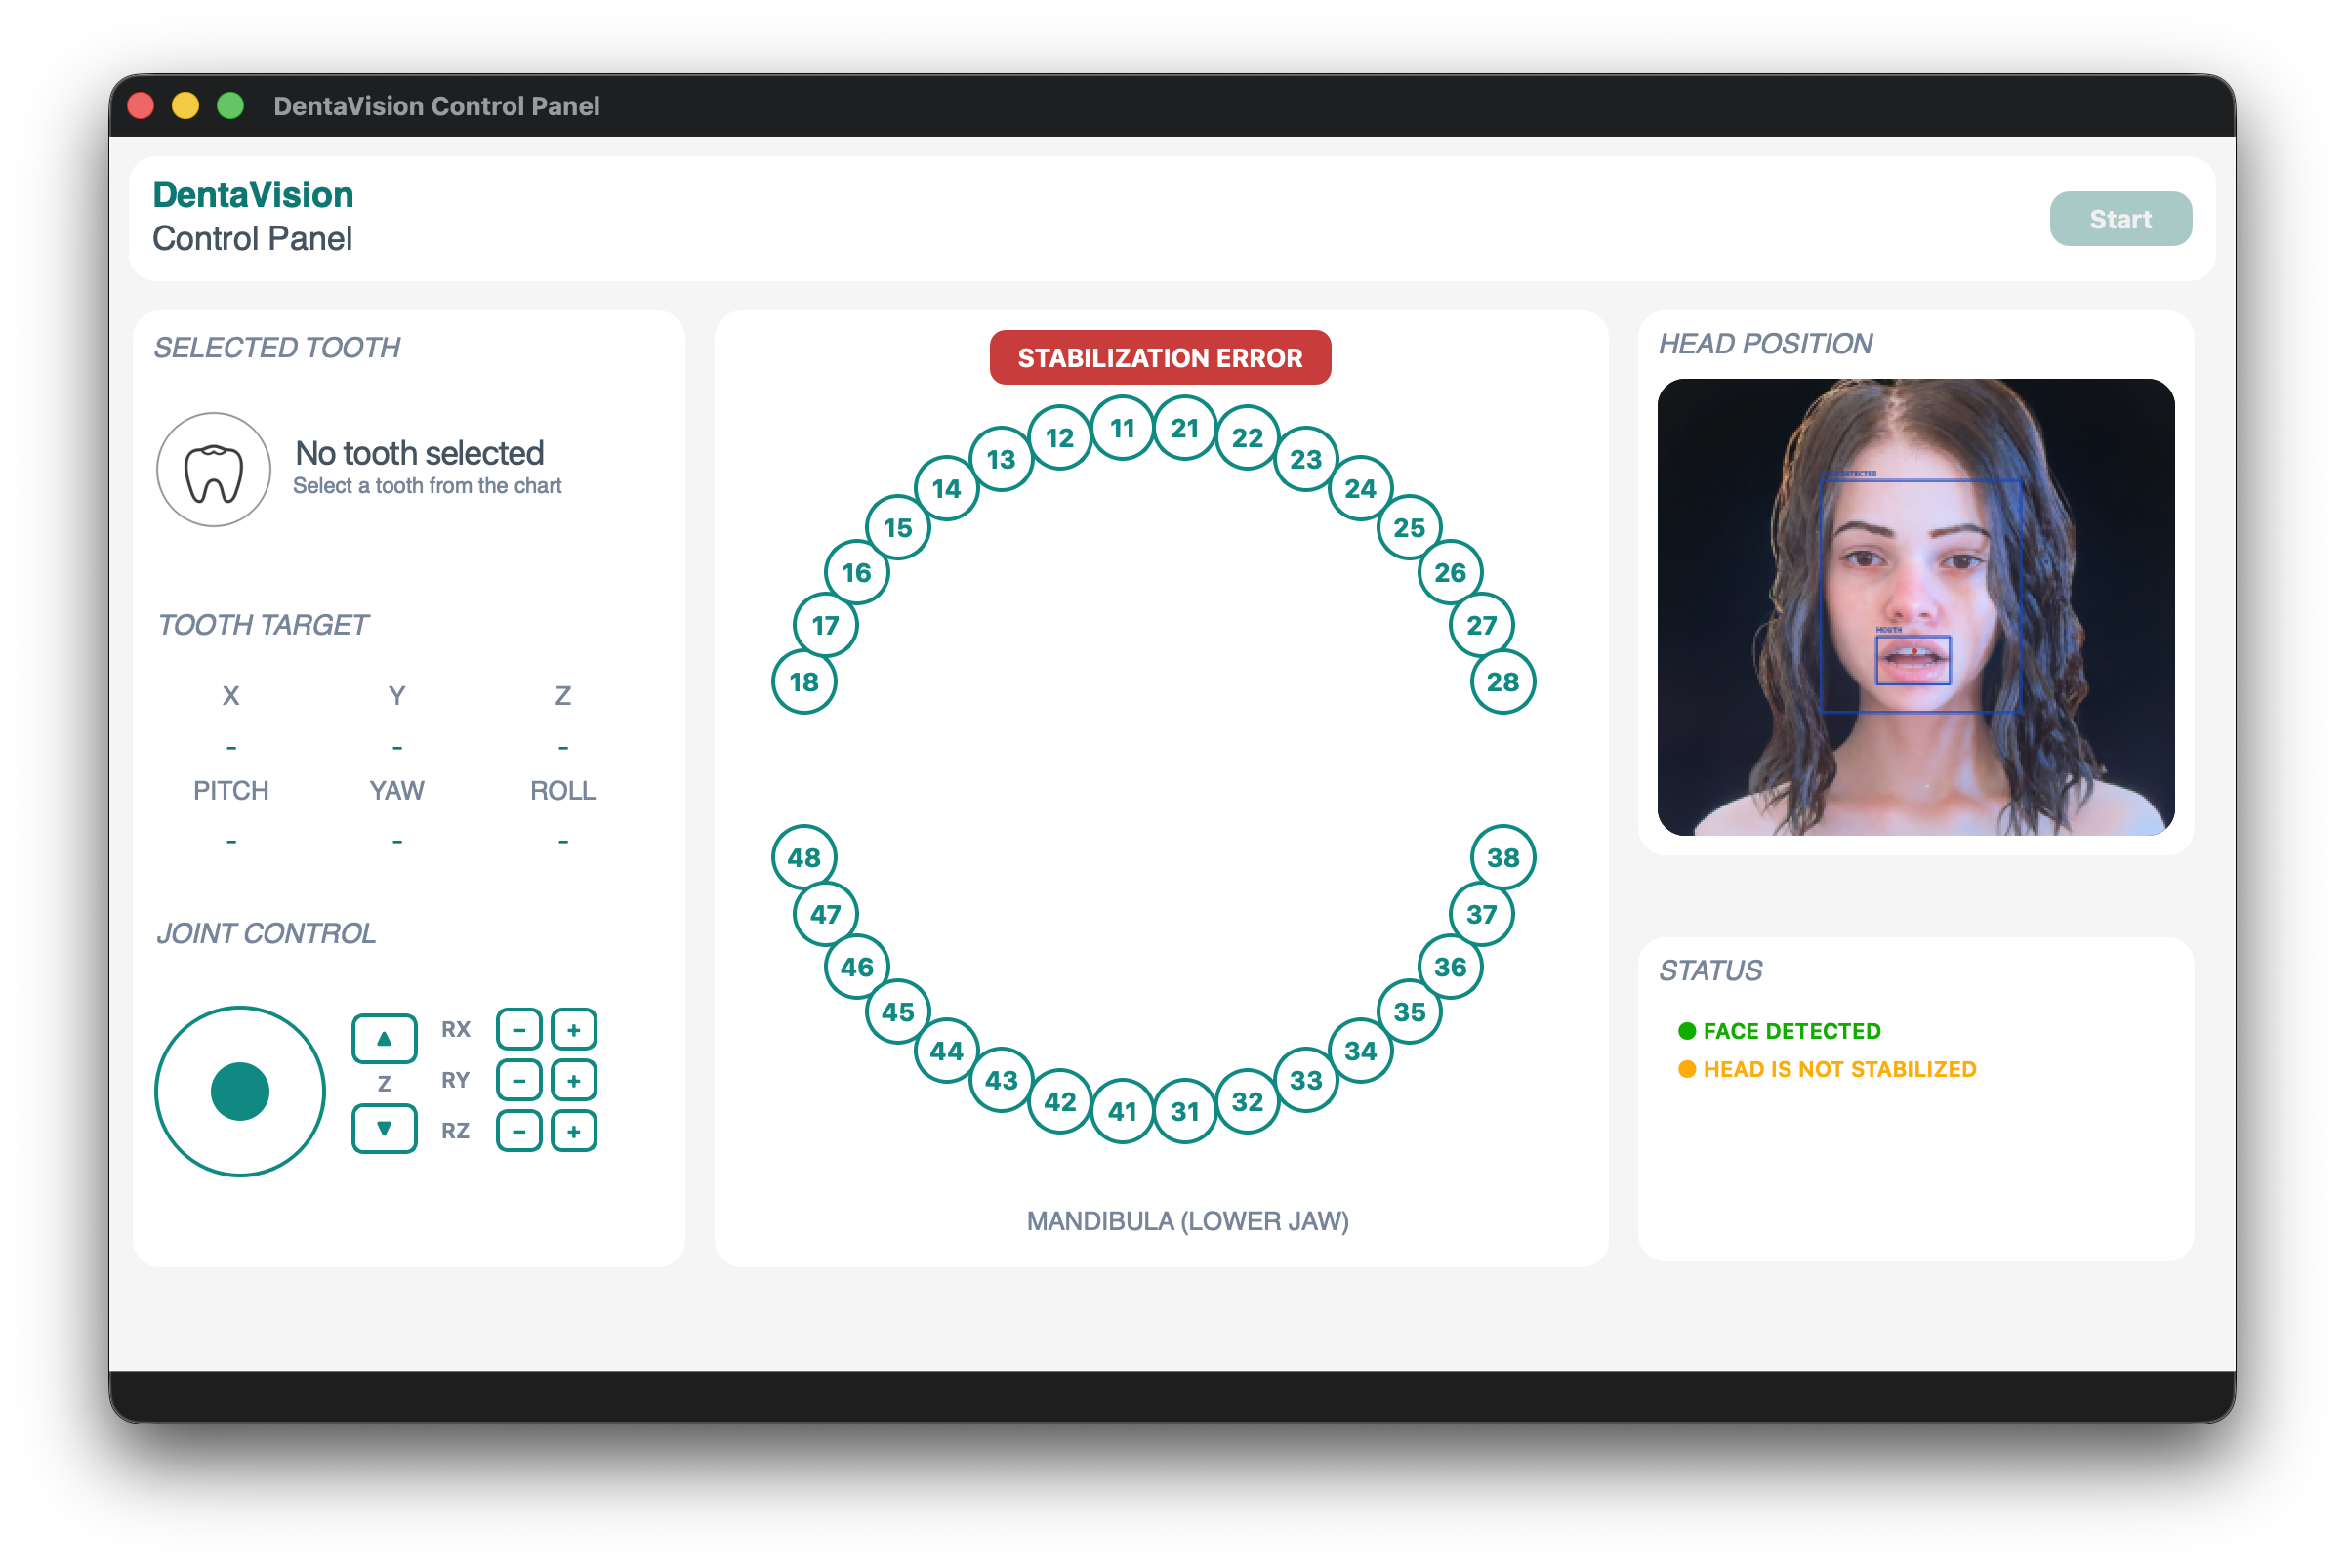
\includegraphics[width=\columnwidth,height=0.45\textheight,keepaspectratio]{ui_assets/demo2-5.png}
    \caption{Demo}
    \label{fig:demo_first}
\end{figure}

\begin{figure}[t]
    \centering
    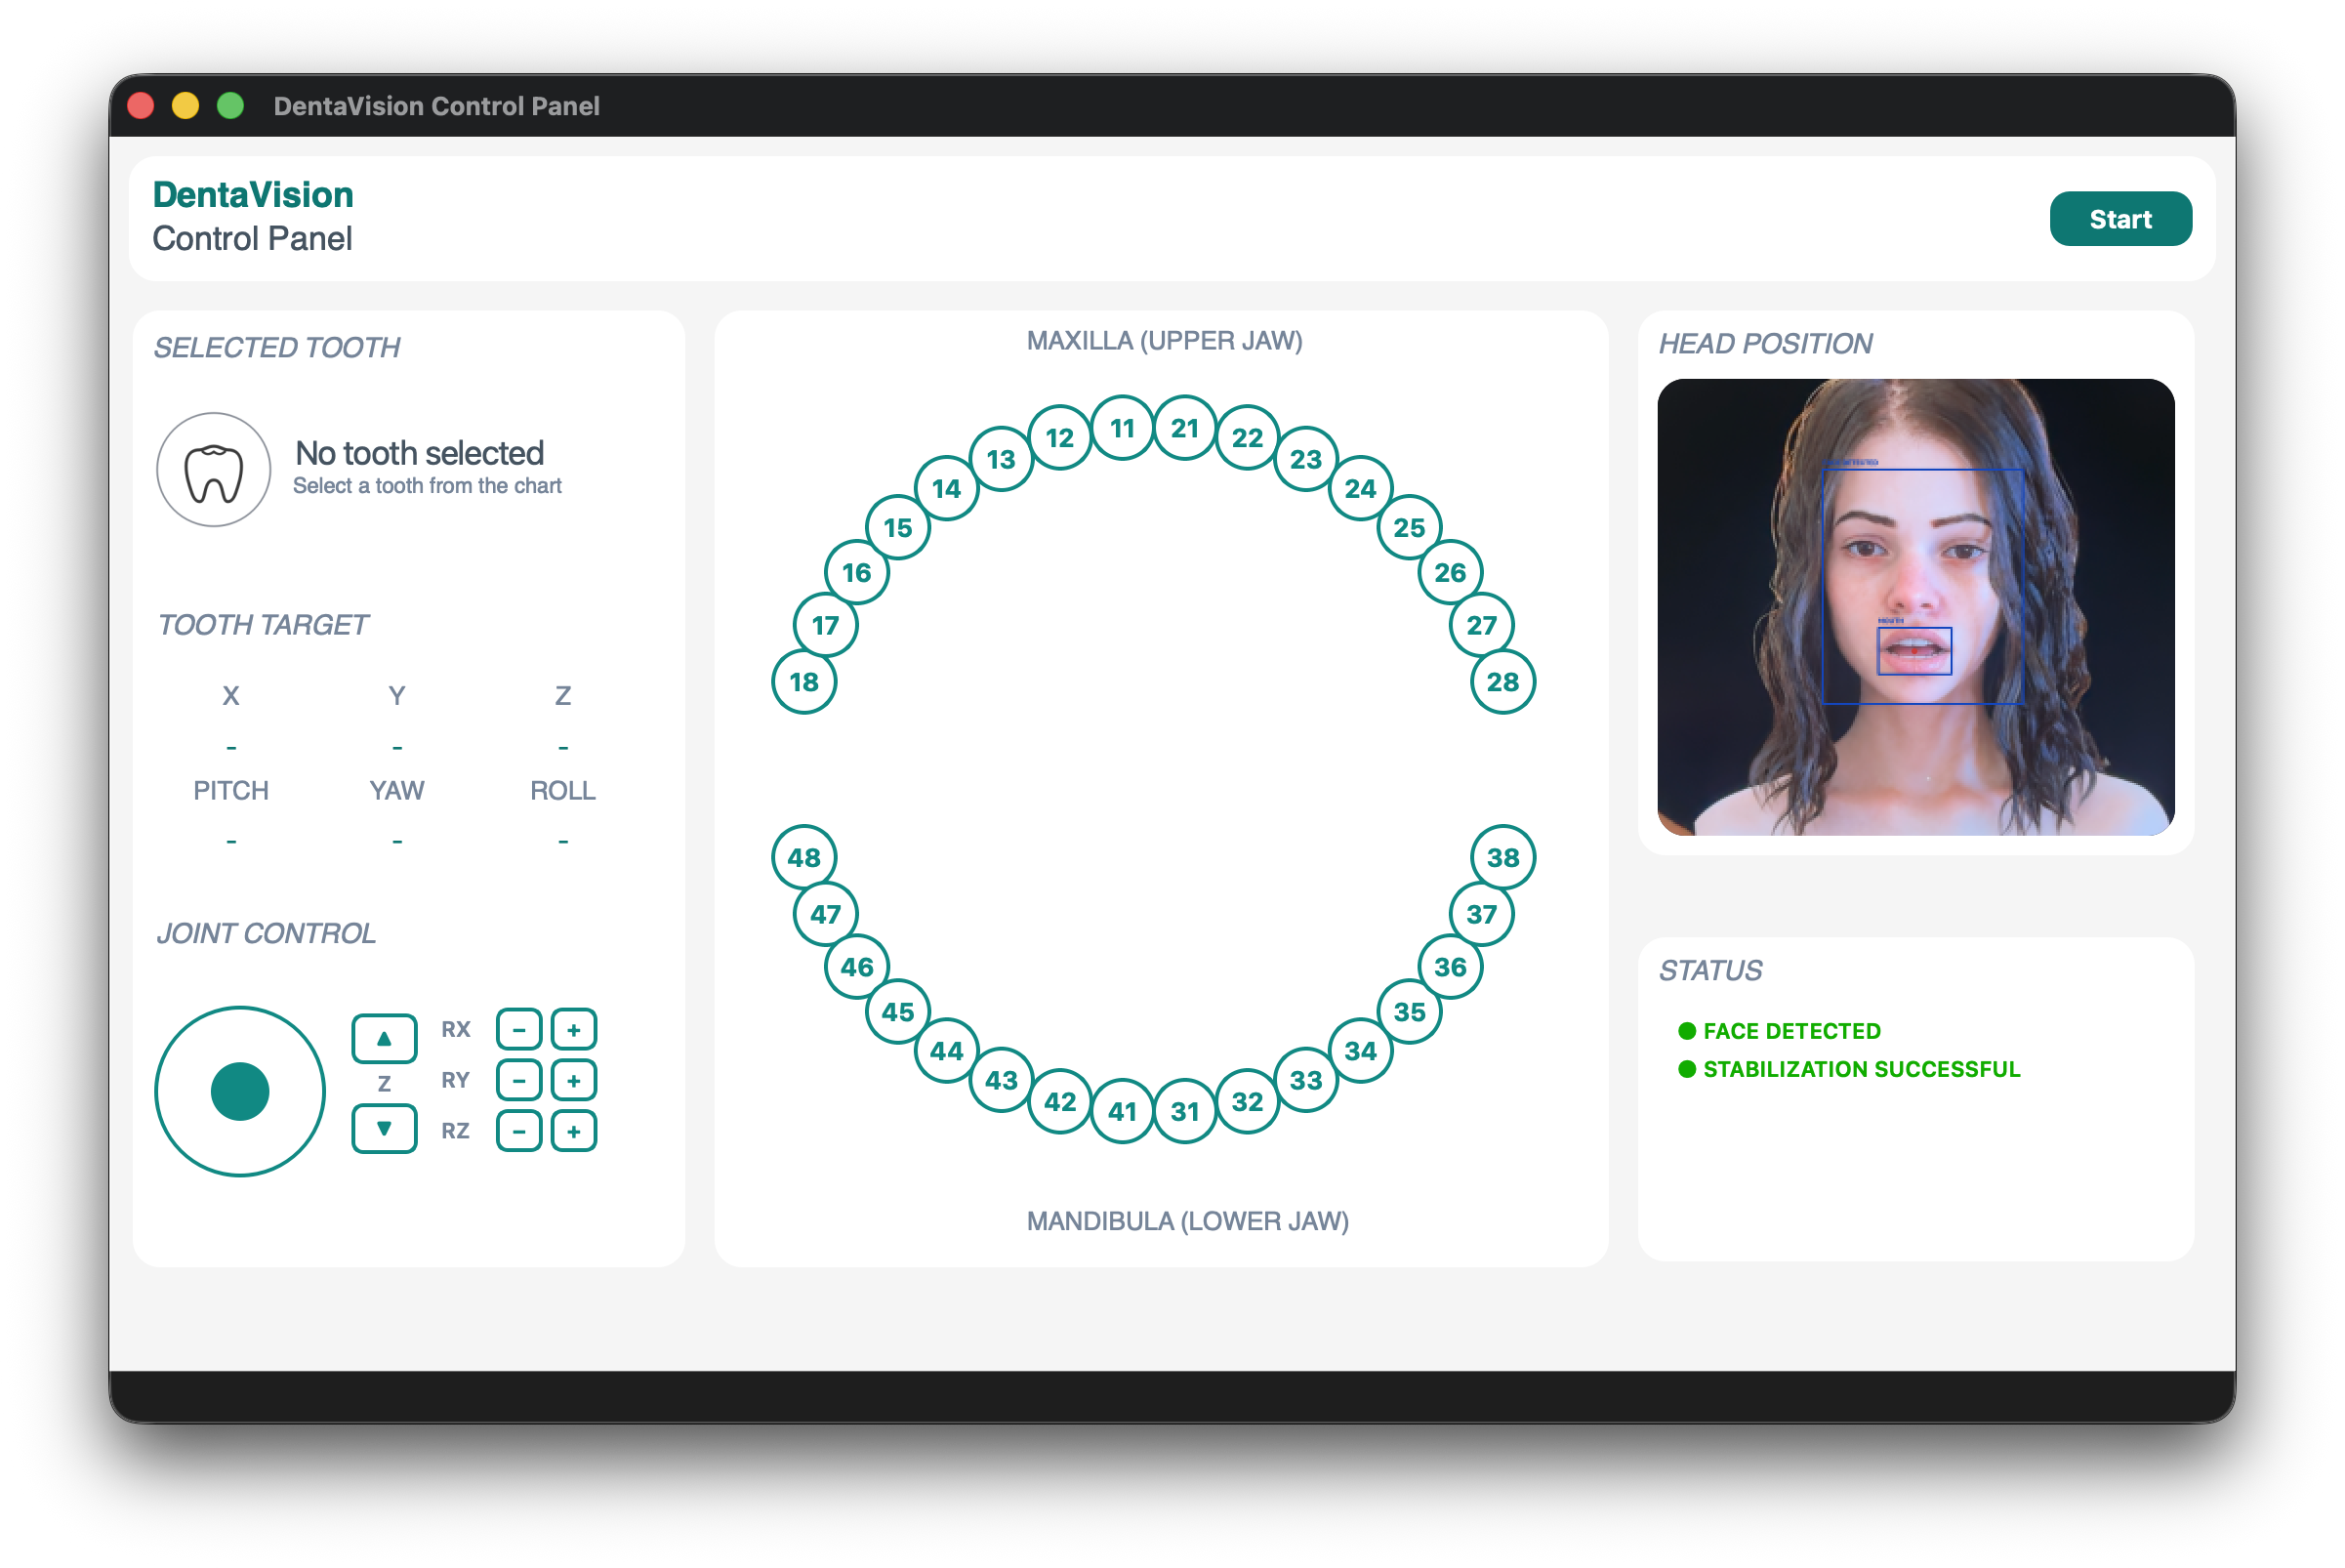
\includegraphics[width=\columnwidth,height=0.45\textheight,keepaspectratio]{ui_assets/demo3.png}
    \caption{Demo}
    \label{fig:demo_second}
\end{figure}

\begin{figure}[t]
    \centering
    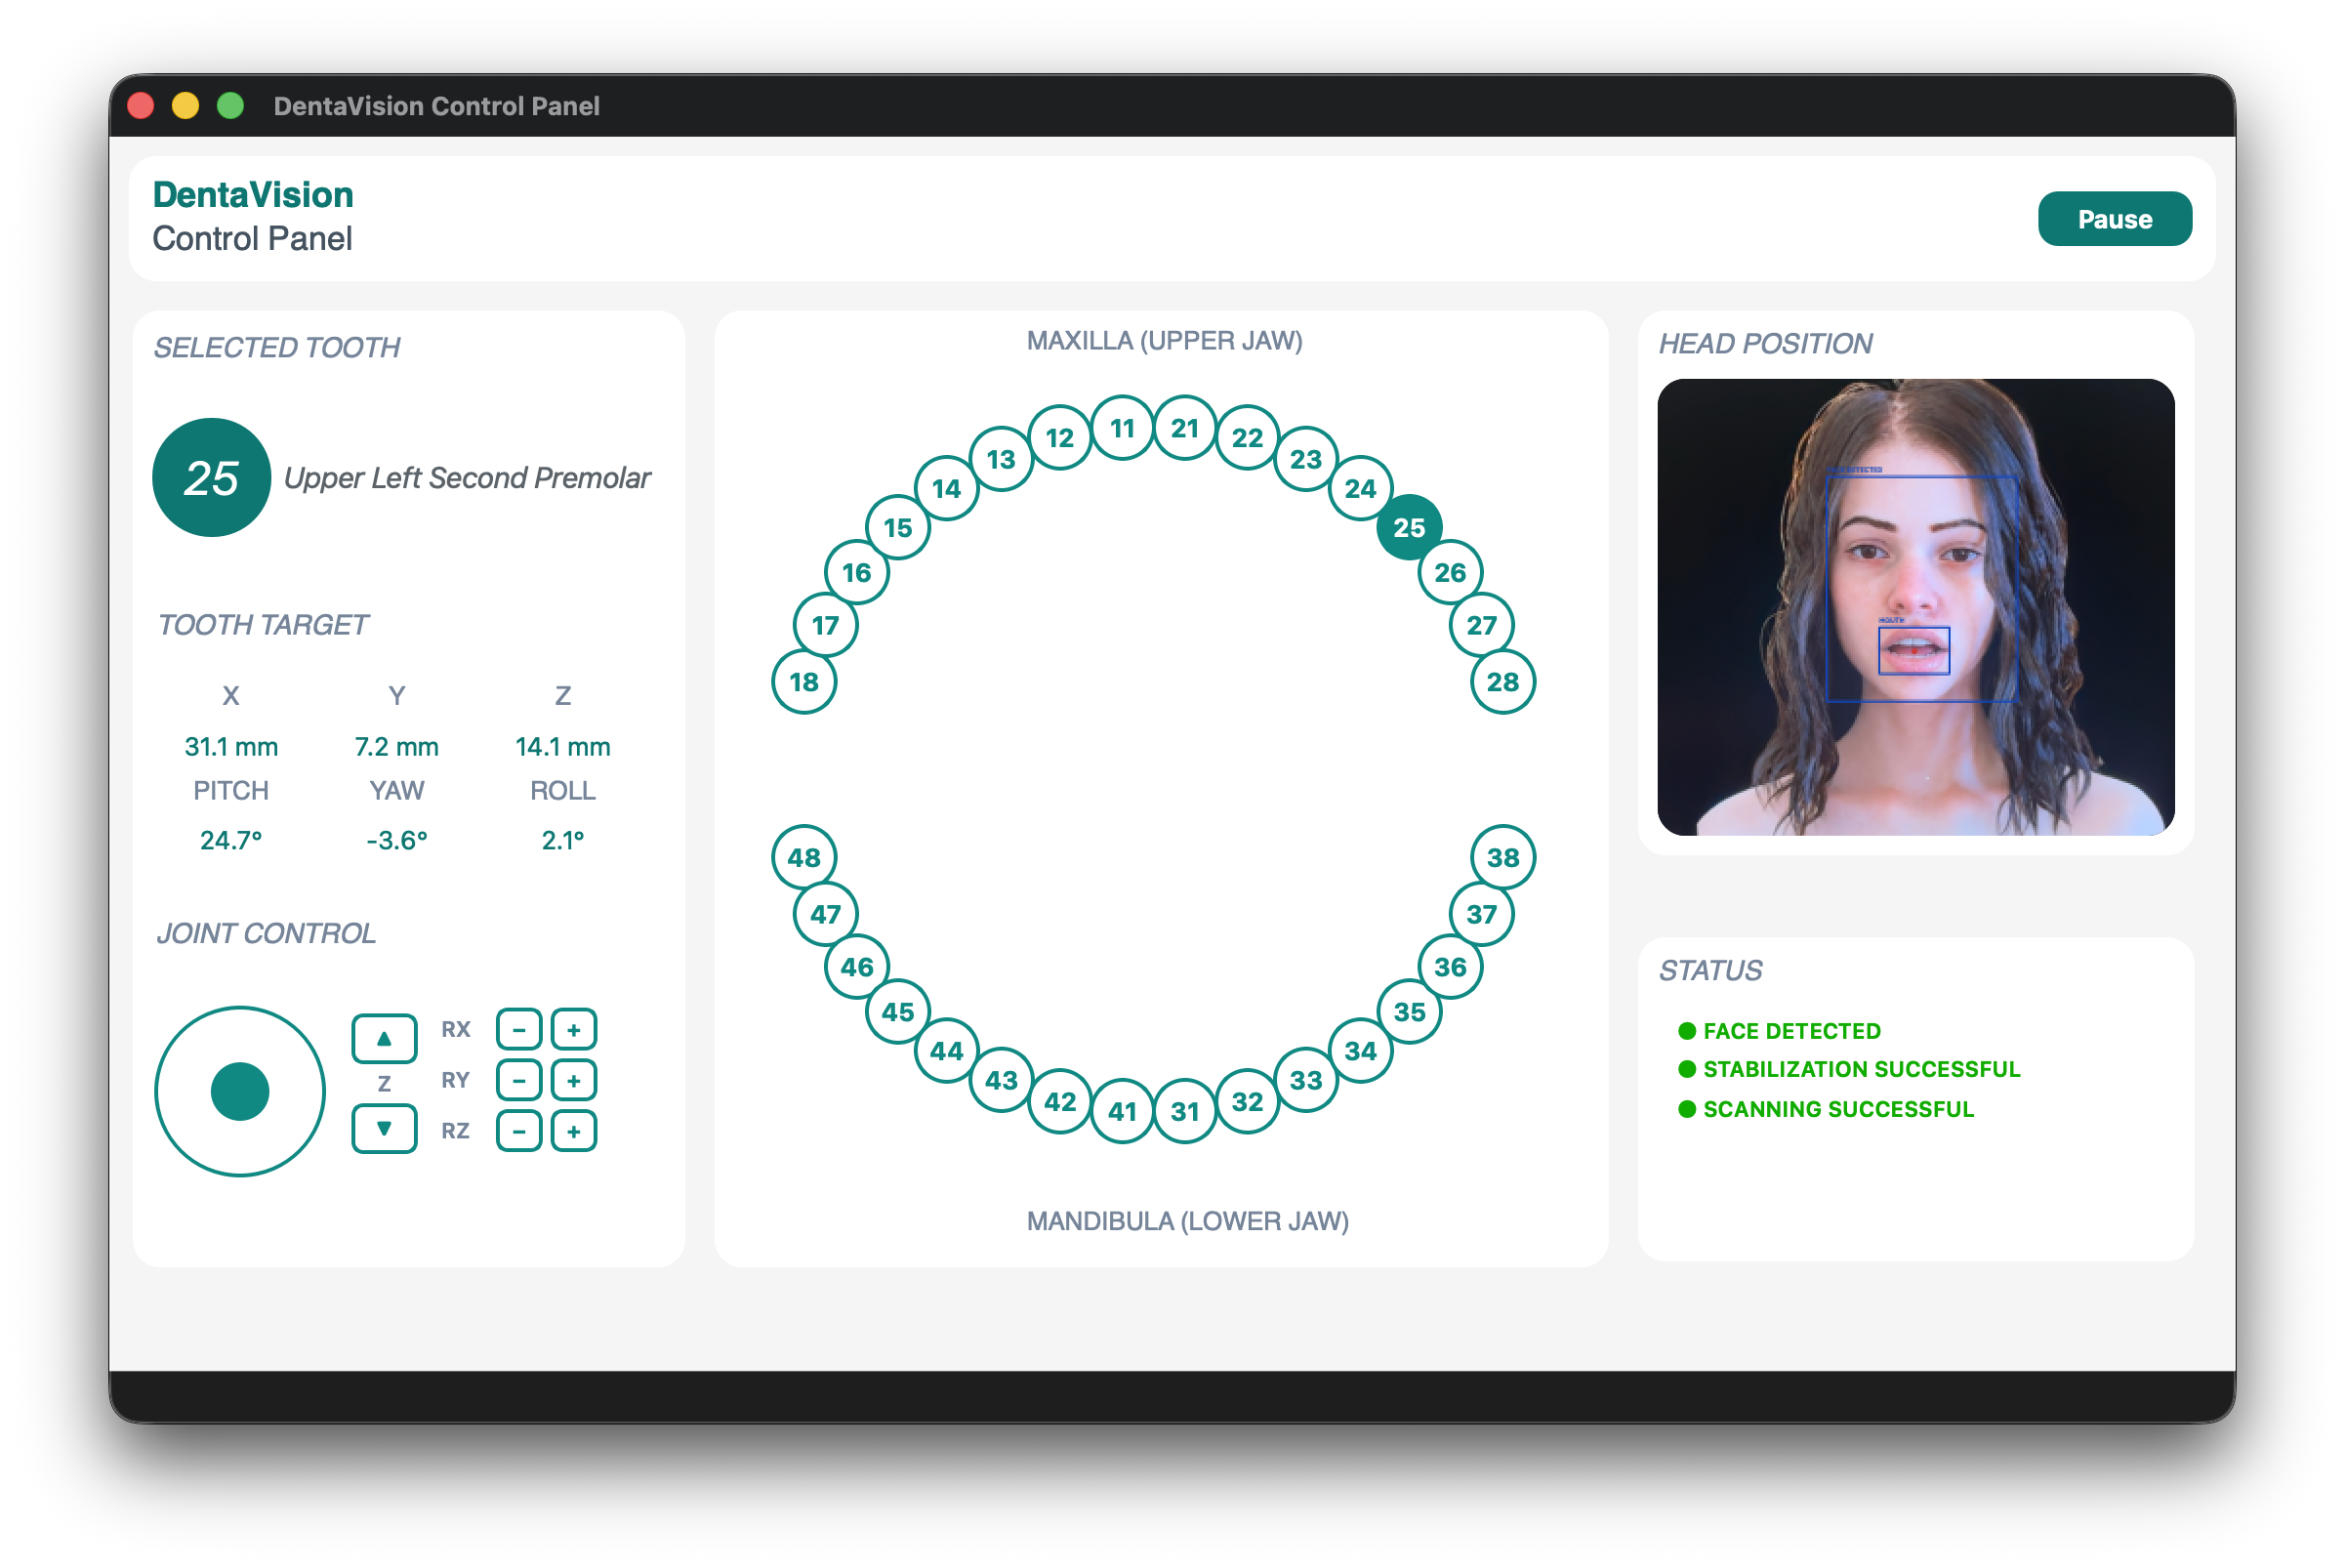
\includegraphics[width=\columnwidth,height=0.45\textheight,keepaspectratio]{ui_assets/demo4.png}
    \caption{Demo}
    \label{fig:demo_third}
\end{figure}

\begin{figure}[t]
    \centering
    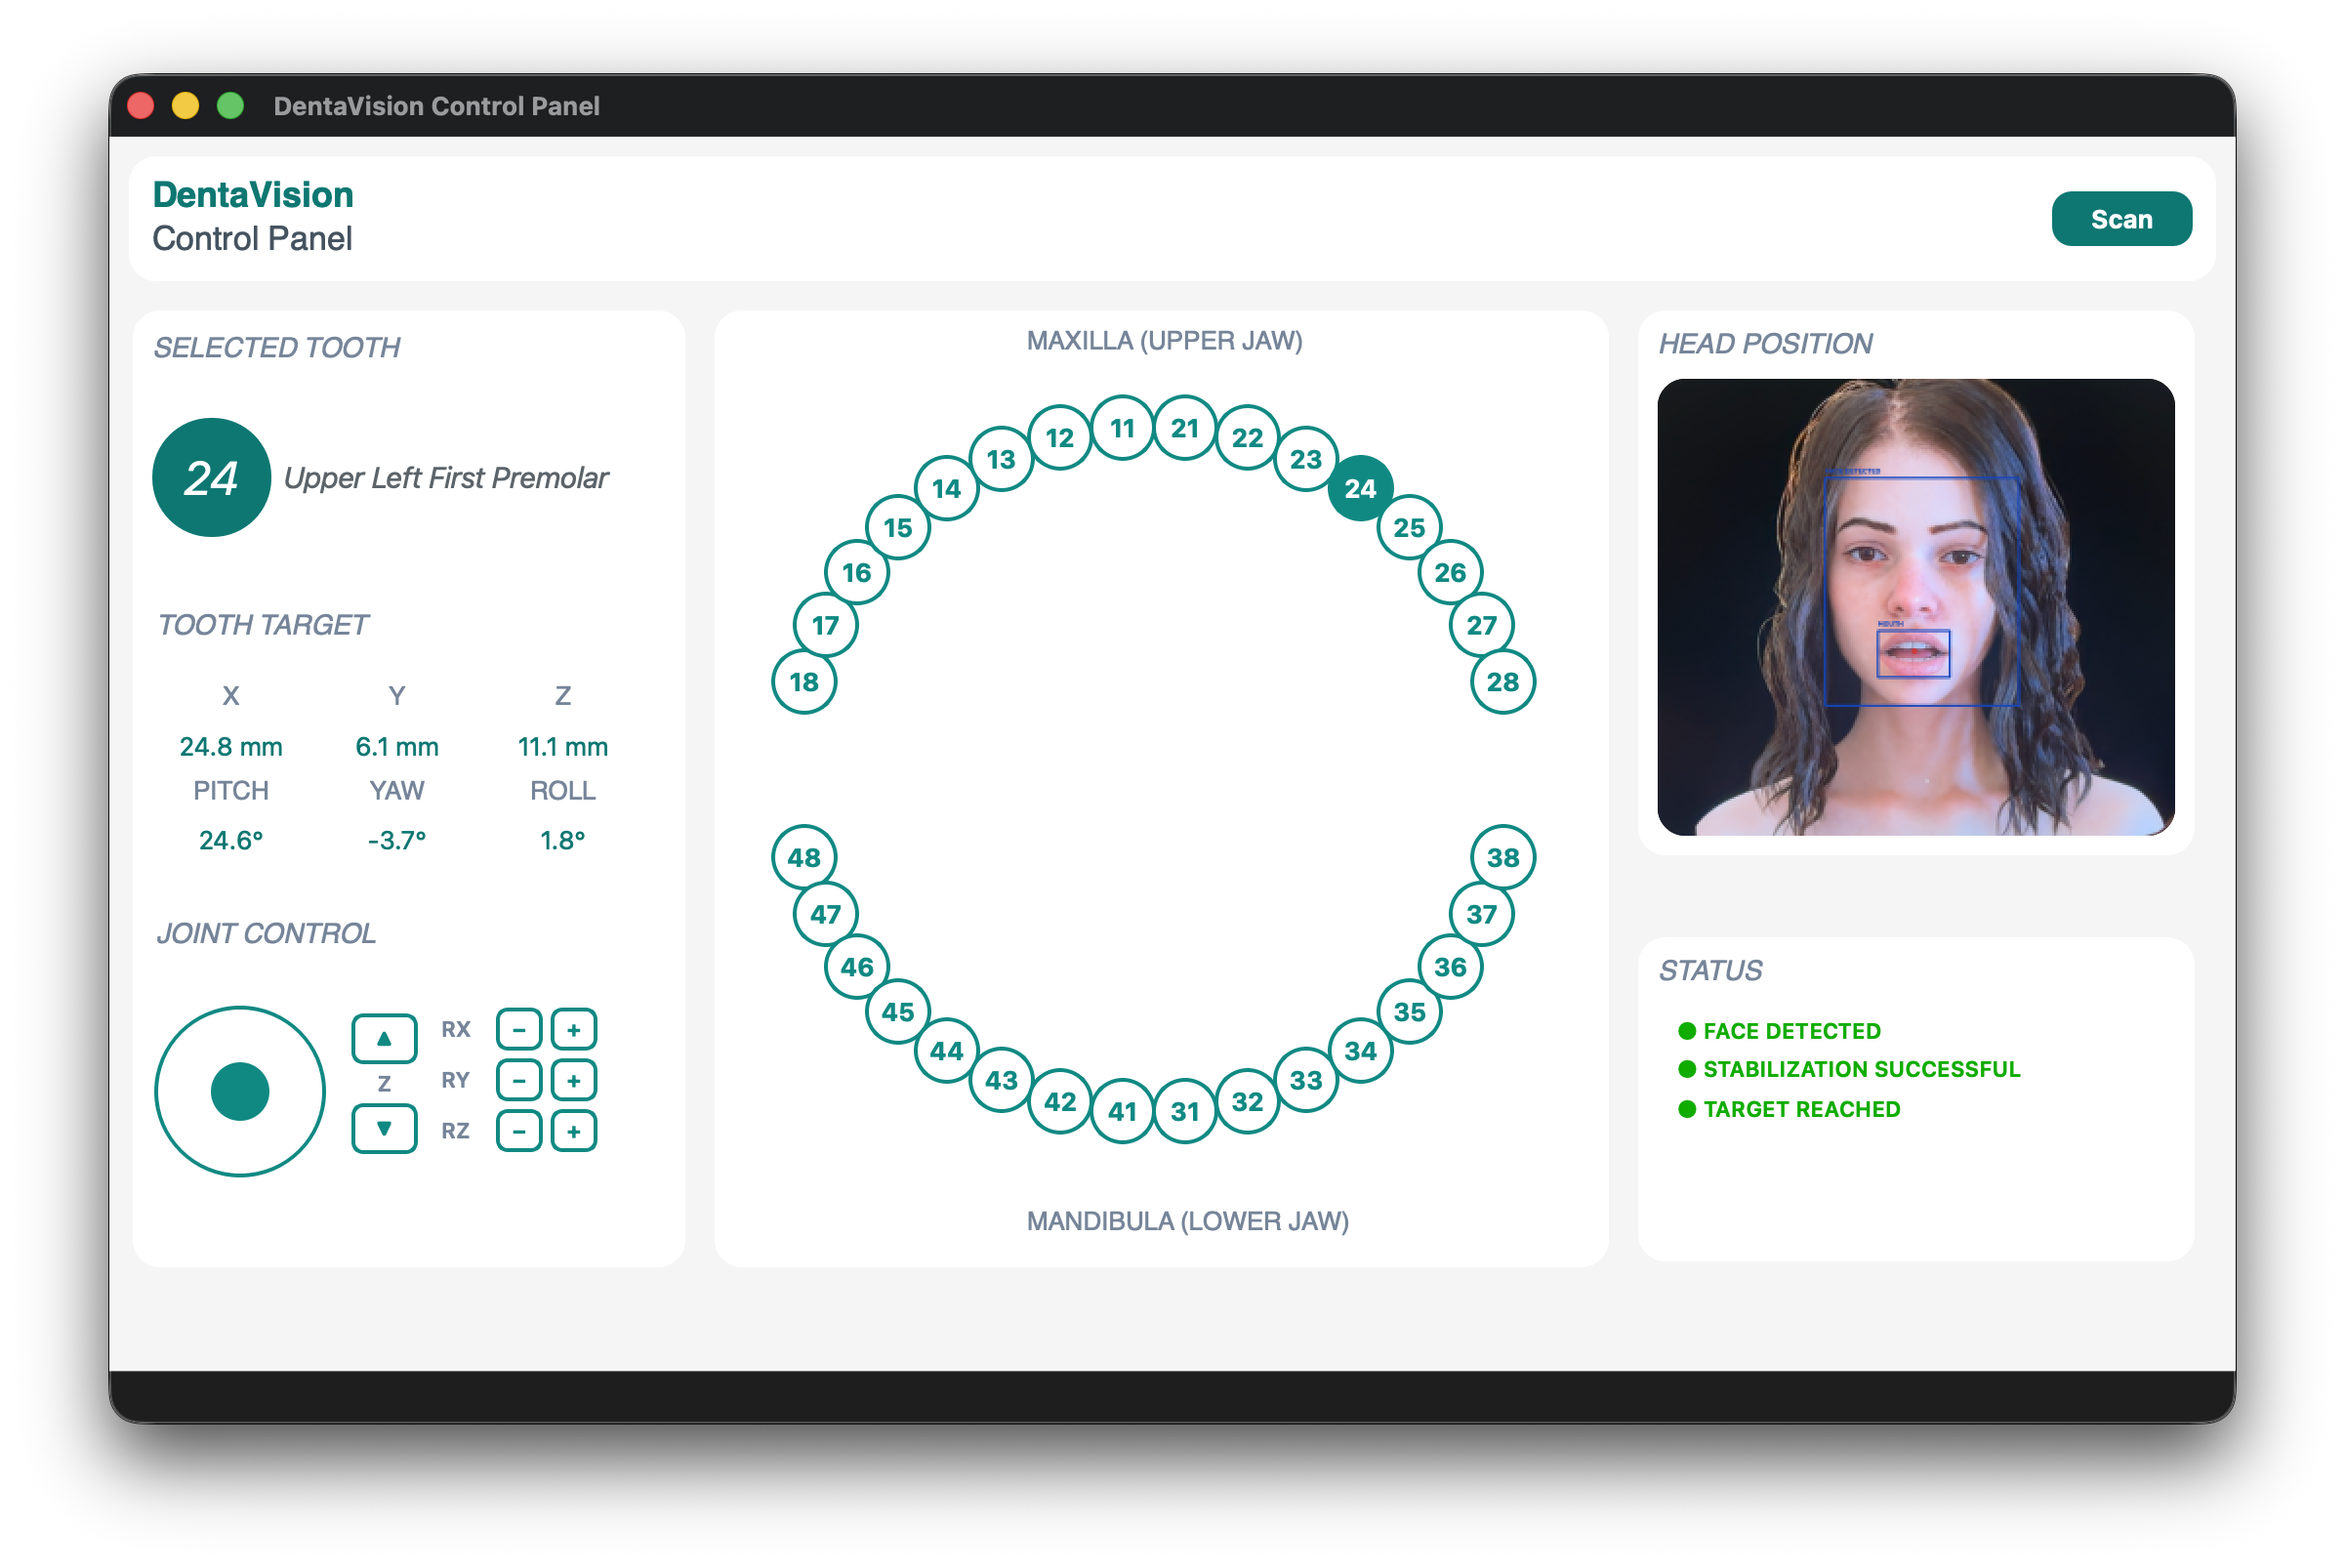
\includegraphics[width=\columnwidth,height=0.45\textheight,keepaspectratio]{ui_assets/demo4_6.png}
    \caption{Demo}
    \label{fig:demo_fourth}
\end{figure}

\section{Future Implementations}

